\documentclass[reprint,amsmath,amssymb,aps,pre]{revtex4-1}
% Latex
\usepackage[english]{babel}
\usepackage[utf8]{inputenc}
\usepackage[T1]{fontenc}
% Xelatex
%\usepackage{polyglossia}
%\usepackage{fontspec}
%\setdefaultlanguage{english}
%\setmainfont{DejaVu Sans}
%\setsansfont{DejaVu Sans}
%\setmonofont{DejaVu Sans Mono}
\usepackage{bm}
\usepackage{cleveref}
\usepackage{xcolor}
\usepackage{algpseudocode}
\usepackage{graphicx}
\usepackage{subfigure}

\definecolor{light-gray}{gray}{0.95}
\newcommand{\code}[1]{\colorbox{light-gray}{\texttt{#1}}}
% When cleveref fails to do its job
\newcommand{\apref}[1]{Appendix \ref{#1}}

\begin{document}
%*Corresponding author: Kirill M. Gerke, Tel.: +79661877715, E-mail: kg@ifz.ru,
%Address: Schmidt Institute of Physics of the Earth of Russian Academy of
%Sciences, Bolshaya Gruzinskaya str. 10/1, Moscow, 123242, Russia
\author{Aleksei I. Samarin}
\altaffiliation{Computational Mathematics and Cybernetics, Lomonosov Moscow
  State University, Moscow, 119991, Russia}
\affiliation{Schmidt Institute of Physics of the Earth of Russian Academy of
  Sciences, Moscow, 123242, Russia}
\author{Vasily Postnicov}
\affiliation{Schmidt Institute of Physics of the Earth of Russian Academy of
  Sciences, Moscow, 123242, Russia}
\author{Marina V. Karsanina}
\affiliation{Schmidt Institute of Physics of the Earth of Russian Academy of
  Sciences, Moscow, 123242, Russia}
\author{Efim V. Lavrukhin}
\altaffiliation{Computational Mathematics and Cybernetics, Lomonosov Moscow
  State University, Moscow, 119991, Russia}
\affiliation{Schmidt Institute of Physics of the Earth of Russian Academy of
  Sciences, Moscow, 123242, Russia}
\author{Kirill M. Gerke}
\email[E-mail:]{kg@ifz.ru}
\affiliation{Schmidt Institute of Physics of the Earth of Russian Academy of
  Sciences, Moscow, 123242, Russia}

\title{Robust surface correlation functions evaluation from discrete digital
  images}

\begin{abstract}
  What have we done?
\end{abstract}

\maketitle

% Write the content here!
\section{Background and motivation}
Correlation functions (CFs) are invaluable universal descriptors of
structure and in this context are utilized in a multitude of scientific
disciplines: material sciences \cite{Cecen}, rock physics, soil physics
\cite{Euras2012;PLoS_ONE;KarsaninaEJSS} and hydrology \cite{Schluter}, cosmology
\cite{oldJap} and food engineering \cite{Antonio}, to name just a handful. As
such, CFs were used to characterize the morphology \cite{tensorPRE} and
representativeness via correlation lengths \cite{Capek,Adler-Thovert}, compare
structures \cite{recons;REVpaper}, compress structural information
\cite{SciRep;Havelka}, describe structural dynamics \cite{Jiao_dynamo;PLoS_ONE},
extract features for deep learning \cite{Tahmasebi;Torq_SciRep;KarsaninaEJSS},
perform stochastic reconstructions
\cite{Adler;Y-T1998;EPL;Jiao;TahmasebiPRL;ourPRL} and fuse multi-scale images
\cite{SciRep;Jiao_multi;Karsanina2018;Tahmasebi2018}. Stochastic reconstruction
is a special topic of interest, as this approach allows to solve an inverse
problem and recover structure from a known set of correlation functions – and
this ability for recovery is the basis for majority of potential usages in the
list above. Early reconstruction techniques mainly involved two-point
probability $S_2$ function, but were improved to include lineal $L_2$ function
\cite{Y-T3D;Capek}, cluster $C_2$ function \cite{JiaoPNAS;JiaoChawla} and
surface-surface $F_{ss}$ function \cite{JiaoPNAS}. With the proper handling
\cite{EPL2} it is possible to incorporate numerous CFs into a reconstruction
procedure. Increasing the number (and order) of functions leads to higher
information content of the CFs set \cite{Gommes1-2}, thus, it allows to
reconstruct and perform stationarity/representativeness characterization
\cite{REV_paper;newPRL} for structures of any complexity.

There are two ways to obtain correlation functions for a given structure at hand
-- either measure them experimentally with the help of scattering intensity
\cite{Debye;Jiao_XCT}, or measured from images. The first approach suffers from
the limitation of CFs that can be obtained this way \cite{Gommes_notchord},
while the second one provides information with limited resolution or/and
resolution to field-of-view ratio \cite{SciRep}. Moreover, the most useful imaging
methods such as X-ray computed tomography (XCT) and scanning electron microscopy
(SEM) due to their underlying physical principles provide gray-scale images
which need to be segmented \cite{Schluter_review} into constituent phases before
CFs computation. It is important to note that such gray-scale images do not
represent phases spatial distribution, but, for example, X-ray spatial
attenuation or electron back-scattering intensities. However, if properly
segmented, high-resolution digital images do provide a possibility to compute
any correlation function. Experimental measurements using small angle scattering
(SAS) are traditionally used to evaluate $S_2$, but it is also possible to
relate scattering intensities to surface correlation functions
\cite{Ma_Torq+inthere}. It would be of great practical importance to obtain
surface correlation functions from both SAS and imaging (focused ion beam
milling combined with SEM allows to obtain the finest imaging resolutions
comparable to SAS and sample CFs from polished surfaces as opposed to surface
imaging \cite{FIB-SEM_paper}) to estimate coefficients for surface and bulk
scattering (see Eq.13 in \cite{Ma_Torq}). But there is a catch -- SAS possesses
close to infinite surface resolution as opposed to digital pixelized images with
inherent segmentation problems due partial volume effects, something we discuss
next.

Recently, Ma and Torquato \cite{Ma_Torq} laid foundation to precise surface
correlation function computations and showed the usefulness of these CFs
evaluation for numerous problems. They have implemented an elegant solution with
the help of infinite resolution random fields that allows finding an exact
intersection with the sampling line. In addition, they also showed that surface
CFs for digital images can be computed by converting integer fields (i.e.,
location of the phases) to float fields with the help of Gaussian filter
\cite{Ma_Torq}. Unfortunately, their solution is not readily applicable to the
majority of structure samples due to non-singularity in their chemical
constitution. The reason is the difference between the contour and real
interface between different phases within the material due to the partial volume
effects \cite{Wildenschild_Sheppard} for XCT imaging -- the presence of multiple
phases within the same pixel/voxel. In other words, the attenuation is a
function of both density and atomic number, which usually are distributed
non-uniformly below the XCT imaging resolution. Somewhat similar is also
relevant for SEM imaging, as secondary or back-scattered electrons are
effectively a convolution of partial signals coming from different depths
\cite{Bultreys_review}. The exact sub-voxel thresholding based on gray-scale
image (similar to the technique used in \cite{Ma_Torq}) is only available in
case it is monomineral. i.~e., the solid phase consists of a completely
chemically homogeneous substance that contrasts perfectly with air/vacuum filled
pore phase -- this is rarely the case for natural materials. All these and
additional problems (such as, for example, experimental noise and artifacts from
inverse Radon transform) arising during gray-scale image processing as related
to image segmentation were extensively discussed elsewhere
\cite{Safonov;Lavrukhin2021}. In other words, we still lack a robust and
computationally effective procedure to evaluate surface CFs from general 2D and
3D images of heterogeneous materials.

In this paper we build upon foundational work of Ma and Torquato \cite{Ma_Torq}
and develop a robust and efficient approach to compute surface correlation
functions from digital 2D and 3D images. The rest of the manuscript is organized
as follows: in \cref{sec:details} we provide all methodological details for
surface CFs computation including analytical solutions to verify the proposed
methodology and describe an image library for extensive testing of our
algorithms. \cref{sec:results} presents all major results of surface functions
evaluations. We discuss obtained results, including the effects of image
scaling, and outline future uses of surface functions within
\cref{sec:scaling}. The paper concludes with a summary in \cref{sec:summary}.

\section{Methodological details}
\label{sec:details}
\subsection{Correlation functions and definitions}
First, we introduce an indicator function $I^{(i)}(x)$, which describes the
affiliation between local points (pixels for 2D and voxels for 3D digitized
images) of structure under study. For a two-phase (or binary) system
(e.g. solid-pore) the indicator function will take the following form in each
location $x$ in the n-dimensional Euclidean space $\mathbb{R}^n$
\begin{equation*}
  I^{(i)}(x) = \left\{
  \begin{array}{ll}
    1 & \quad x \in V_i \\
    0 & \quad \text{otherwise}
  \end{array}
  \right.
\end{equation*}
where $V_i \subset \mathbb{R}^n$ is the region occupied by phase $i$. For
statistically homogeneous media the ensemble average of $I^{(i)}$ equals volume
fraction of a given phase. For binary media the following equality holds:
\begin{align*}
  \phi_{void} &+ \phi_{solid} = 1 \\
  \phi_i &= \langle I^{(i)}(x) \rangle
\end{align*}
In a similar fashion we can define an interface indicator function $M(x)$ which
provides interface area $s$ if averaged over the whole image:
\begin{align}
  M(x) &= |\nabla I^{(solid)}(x)| =|\nabla I^{(void)}(x)| \label{eq:interface} \\
  \langle M(x) \rangle &= s
\end{align}
The simplest, yet foundational correlation function is two-point probability
function $S_2$ which is defined as a probability to sample the ends of a line
segment within the same phase:
\begin{equation}
  S_2^{(i)}(x_1, x_2) = \langle I^{(i)}(x_1) I^{(i)}(x_2) \rangle \label{eq:twopoint}
\end{equation}
This equation can be further simplified for statistically homogeneous media, as
$S_2$ will dependent only on the relative displacement $r$:
\begin{equation*}
  S_2^{(i)}(x_1, x_2) = S_2^{(i)}(r)
\end{equation*}
Now, analogously to $S_2$ we can define surface-surface and surface-void
correlation functions:
\begin{align}
  F_{ss}(r) &= \langle M(x)M(x+r) \rangle \label{eq:fss} \\
  F_{sv}(r) &= \langle M(x)I^{(void)}(x+r) \label{eq:fsv} \rangle
\end{align}
The value of $S^{(i)}_2(r)$ at zero is a fraction of phase $i$ in a medium:
\begin{equation}
  S_2^{(i)}(0) = \phi_i \label{eq:s2porosity}
\end{equation}

By looking at \cref{eq:twopoint} and \cref{eq:fss}-\cref{eq:fsv} one can observe
some significant similarities between two-point probability and two-point
surface functions (see \cref{fig:scheme}). They will help us in
computations. However, let's first consider major differences. Firstly, unlike
$S_2$ in \cref{eq:s2porosity}, $F_{ss}(r)$ is not defined at $r=0$. $S_2$ can
be viewed as a autocorrelation of the image, i.~e., computing correlations
between shifted realization of the image -- something that can be used to
effectively compute $S_2$ with the help of fast Fourier transform (FFT) on
modern hardware, especially GPUs. If we apply the same analogy \cref{eq:fss}
can be considered as an intersection of the interface with itself for all
possible shifts. But for the correlation length zero this intersection is
technically infinity. While surface-void function is well defined at $r=0$, it
differs from $S_2$ in two significant aspects. Firstly, it mostly resembles
two-point cross-correlation function (as instead of autocorrelation we have to
compute correlation between the interface and the void phase). Secondly, one has
to keep in mind that cross-correlation is not commutative, so we get two
surface-void functions: correlation between an interface and a void phase and
correlation between a void phase and an interface. These considerations will be
very useful in understanding our computational framework. More detailed
information on two-point probability and surface correlation functions can be
found in comprehensive Torquato's book \cite{Torq_book}.

$M(x)$ is basically defined as infinity on the interface and zero elsewhere.
Therefore, it is hard to directly compute $\langle M(x), M(x + r) \rangle$.
We can replace the line of zero width and infinite value 
with a strip of width $\varepsilon$ and value $\frac{1}{\varepsilon}$: $M(x; \varepsilon)$. 
Then $F_{ss}(x; \varepsilon) = \langle M(x; \varepsilon), M(x + r; \varepsilon) \rangle$ 
is simply an intersection area of two strips 
--- original and shifted --- 
multiplied by $(\frac{1}{\varepsilon})^2$. 
And with $\varepsilon \to 0 \Rightarrow F_{ss}(r; \varepsilon) \to F_{ss}(r)$.
Area between two black dashed circles on \cref{fig:Fss-explained} 
represents $M(x; \varepsilon)$,
red is for $M(x + r; \varepsilon)$. 
Blue color marks the intersection area.

\begin{figure}
  \centering
  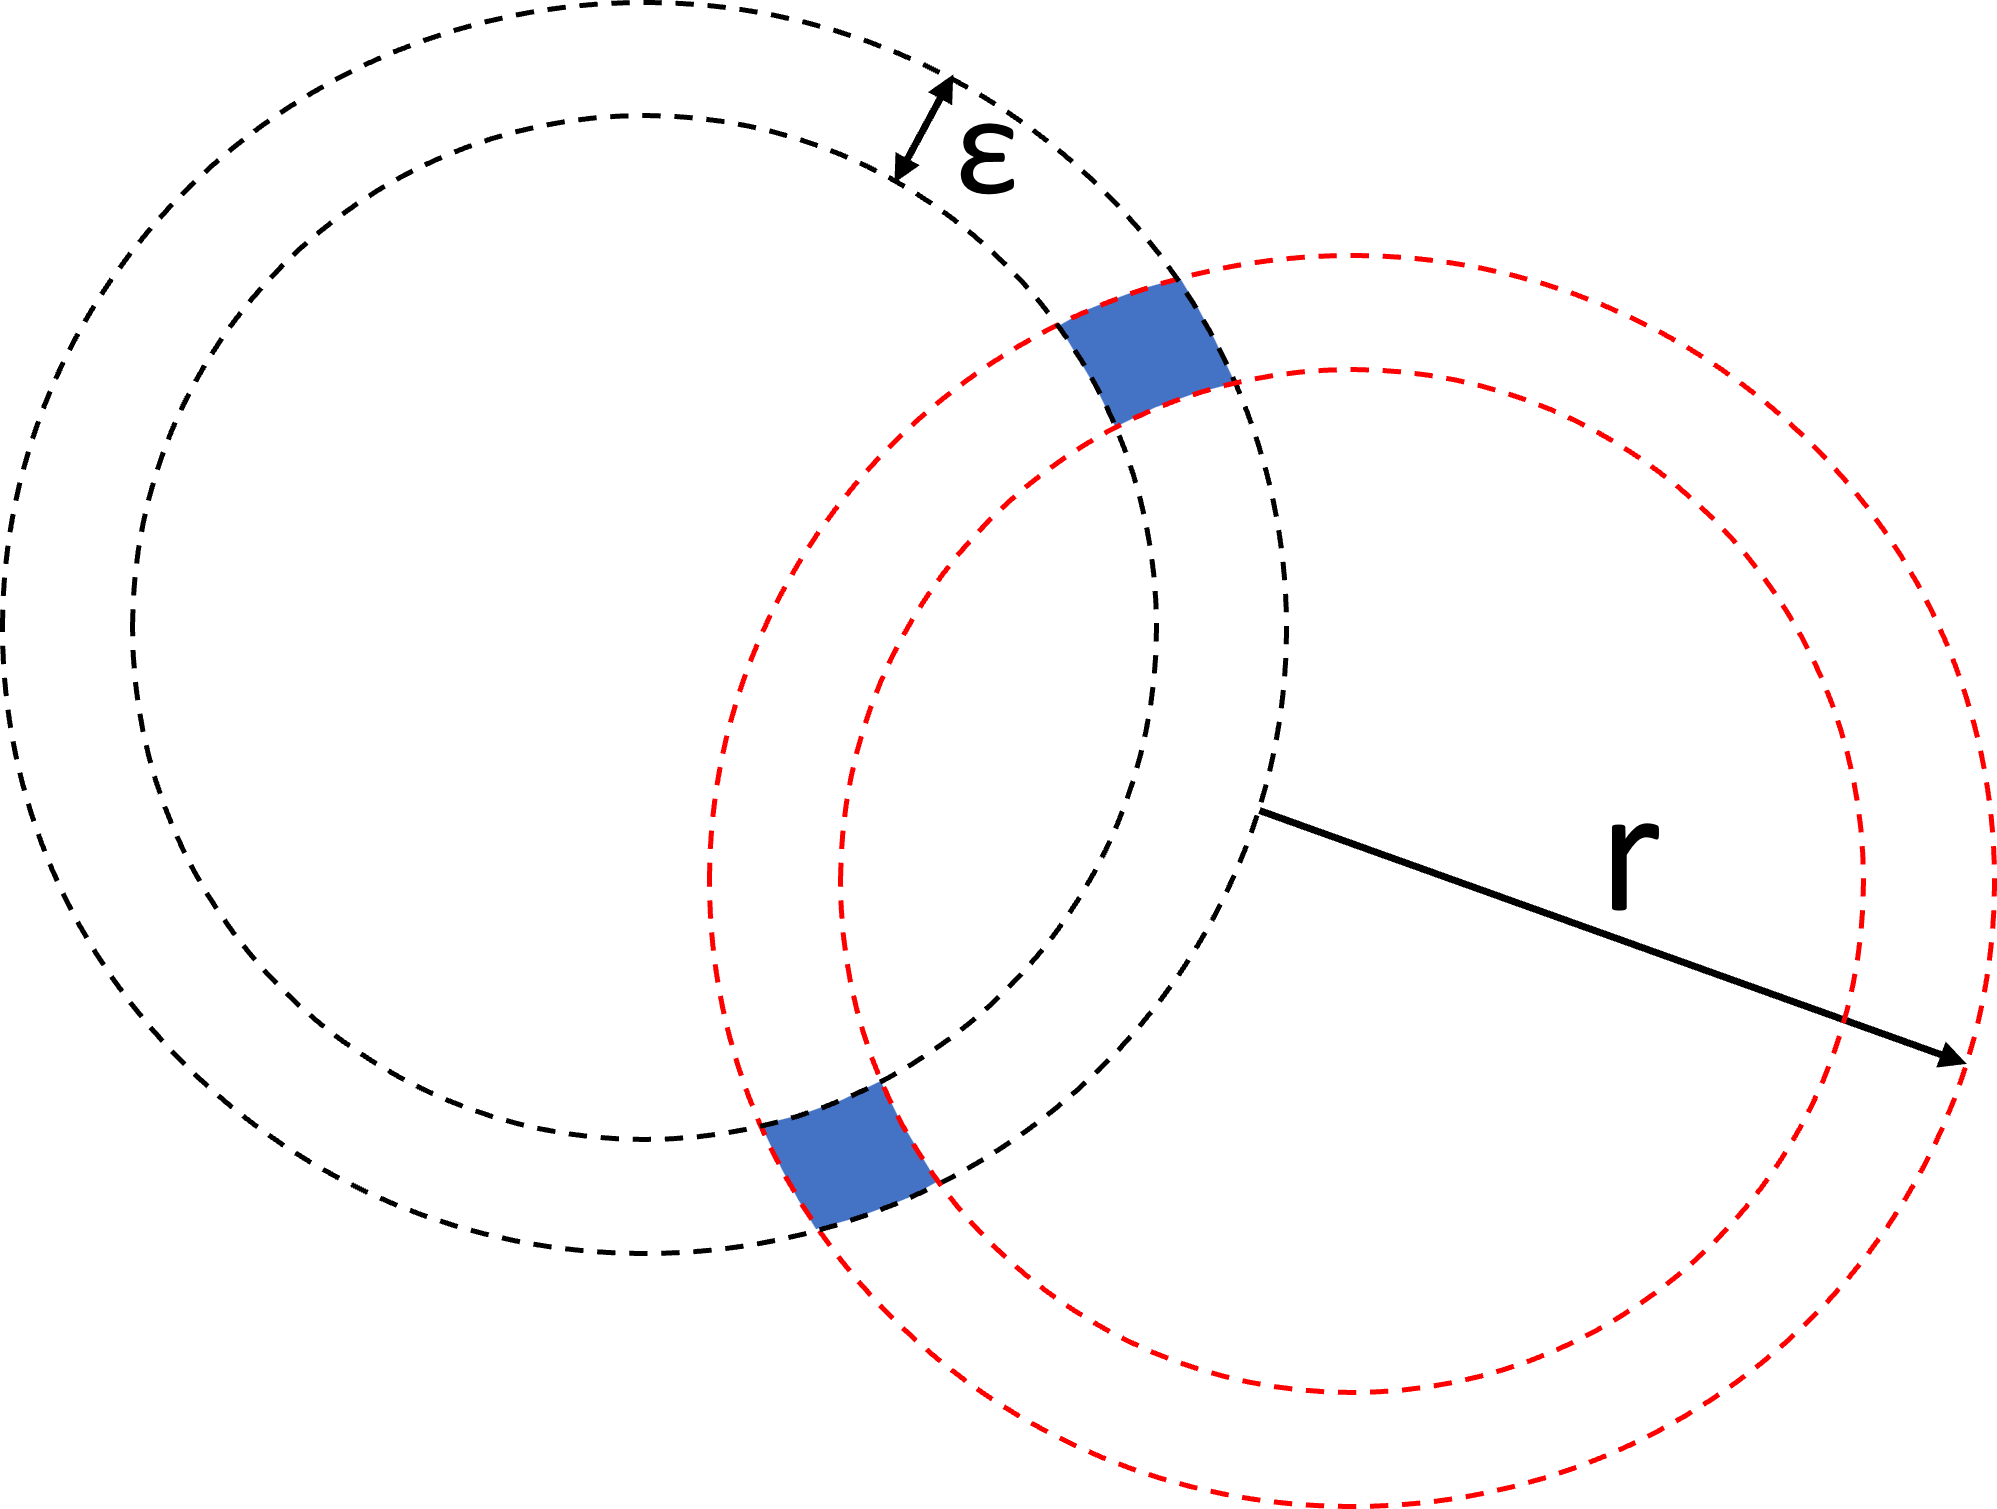
\includegraphics[width=0.9\linewidth]{images/Fss.png}
  \caption[]{Interpretation of $F_{ss}$ as self-intersection of interface.
    \textcolor{red}{Torquato described it as ``previous algorithm'', fig.3}}
  \label{fig:Fss-explained}
\end{figure}


\begin{figure}[ht]
  \centering
  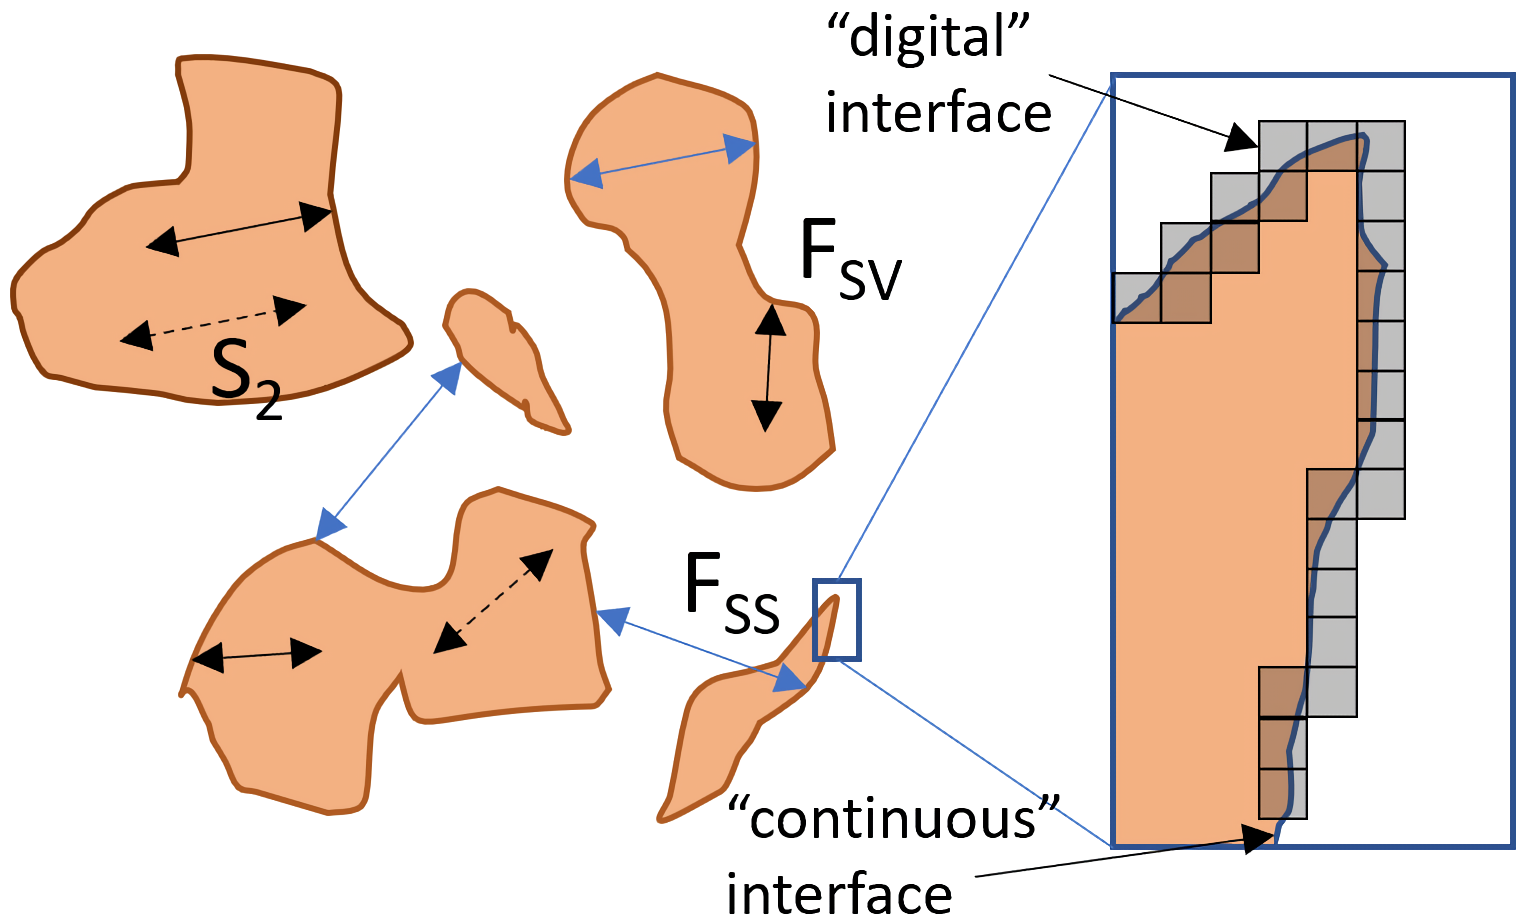
\includegraphics[width=0.9\linewidth]{images/scheme.png}
  \caption[]{A schematic depiction of a binary porous media (pores are shown in
    color) with examples of positive events for surface $F_{ss}$, $F_{sv}$ and
    two-point probability $S_2$ correlation functions. The zoomed in area
    represents the difference between the true ``continuous'' interface in
    between pore and solid phases with pixelized ``digital'' interface emerging
    due to limited resolution of digital images.}
  \label{fig:scheme}
\end{figure}

\subsection{Computation of correlation functions}
One can potentially apply a number of different computational approaches to
evaluate surface functions. We start by exploring the most computationally
straightforward algorithms and move towards more complex ones. \textbf{I cannot
 understand this.} The surface area
in \cref{eq:interface} has infinitesimal volume on digital images. This prevents
the usage of two methods to compute (cross-) correlations: scanning with line
segment and autocorrelation with FFT that are immediately applicable to digital
pixelized/voxelized images. The usage of interfaces between voxels ``as is''
leads to severe errors in $s$ and surface geometry, as known from application of
3D imaging for geometry and topology analysis \cite{AWR_PNM} or energy
minimization problems \cite{jagged_surfaces}. Another option would be to
describe the boundaries between voxels with some curves, e.~g., splines. This
way it would be possible to perform surface CFs sampling by line intersection as
described by Ma and Torquato \cite{Ma_Torq}. While an exact boundary can be
obtained for deterministic structures such as disk/ball packings, splines
would provide only a very approximate solution for the boundaries of arbitrary
digitized structure due to the limit in resolution for a given image
\cite{Eusosoil2012}. In other words, contours extracted from digital images will
approach real boundaries between phases only when the spatial resolution
approaches infinity. But the same is also true for digital pixelized/voxelized
images. Thus, the options to compute surface correlation functions include
``continuous'' approach (such as implemented in \cite{Ma_Torq}) and ``digital''
approach (similar to computation of $S_2$ from digital images) as depicted in
\cref{fig:scheme}.

We adopt the ``digital'' approach, as it is clear that in the limit of infinite
resolution the ``continuous'' approach will not provide any advantages for
arbitrary XCT or SEM images.

%Во всем пейпере надо привести все A, M, Image и т.п. к единообразию тернимологии- а то
%кто в лес, кто по дрова…

\textbf{High-level algorithm}

$F_{ss}$ algorithm:
\begin{enumerate}
    \item reduce multi-phase image $A$ to two-phase image by applying indicator
      function $A'= I(A)$.
    \item extract interface from binary image $A'$ as image of the same size $M = S(A')$
    \item compute auto correlation function of interface $F_{ss} = S_2(M)$
\end{enumerate}

$F_{sv}$ algorithm:
\begin{enumerate}
    \item reduce multi-phase image $A$ to two-phase image by applying indicator
      function $A'= I(A)$.
    \item extract interface from binary image $A'$ as image of the same size: $M = S(A')$
    \item extract void phase from multi-phase image $A$: $V = I^{(void)}(A)$
    \item compute cross correlation function: $F_{sv} = cc(M, V)$
\end{enumerate}

\textbf{Interface extraction}
There are several methods for interface extraction.
We will focus on methods, that construct digital image of the same size.
Pixels (or voxels) take value between $0$ and $1$:
zero value -- inner part of phase, and positive value means pixel lies on the
interface.

\textit{Distance map}.
This method creates binary image. 
The interface between binary phases is represented by a one
pixel thick contour (in two-dimensional case) or one voxel thick surface (in
three-dimensional case). This contour or surface is extracted from either solid
or void phase with the help of distance map transform with subsequent filtering
out of pixels/voxels with distances greater than $1$.

\textit{Image filtering}.
This method creates gray scale image. We use Sobel operator to detect edges of
the image $A'$, later denoted as $\nabla A$: $\nabla A' = S(A')$. We calculate
$\|\nabla A'\|$ element-wise ($\|\cdot\|$ denotes the usual norm on Euclidean
space). This norm can be interpreted as the probability that a point in $A$
belongs to the interface. In a digitized image $\|\nabla A'\|$ can be
represented as an array of floating point numbers having the same shape as an
original image $A$.

\textbf{Computing correlation}
We will describe method of computing cross correlation function between two
images $f$ and $g$: $cross\_correlation(f, g)$. In the case of auto correlation
function we will replace $g$ with $f$. Algorithm is straightforward when
boundary conditions are periodic. For non-periodic boundary conditions we will
need a minor change.

\textit{Periodic boundary condition}
\begin{enumerate}
    \item compute Fourier transform of input images: $F = fft(f), G = fft(g)$
    \item take complex conjugation from elements of G: $G'[i, j] = \bar{G}[i, j]$
    \item multiply elements of $F$ by elements of $G'$: $CC[i, j] = F[i, j] G'[i, j]$
    \item compute inverse Fourier transform: $cc = ifft(CC)$
    \item divide the resulting matrix by the number of pixels: $cc[i, j] = cc[i, j] / (n m)$
\end{enumerate}

\textit{Non-periodic boundary condition}
\begin{enumerate}
    \item Expand input images by a factor of two, padding new elements with
      zeros ($f^e, g^e$). If the length of the image was $n$, then the length of
      the expanded image will be $2n - 1$, where the last $n - 1$ values will be
      zero. Similarly for the width and height of the image.
    \item compute Fourier transform of expanded images: $F = fft(f^e), G = fft(g^e)$
    \item take complex conjugation from elements of G: $G'[i, j] = \bar{G}[i, j]$
    \item multiply elements of $F$ by elements of $G'$: $CC[i, j] = F[i, j] G'[i, j]$
    \item compute inverse Fourier transform: $cc = ifft(CC)$
    \item circle shift $cc$ by $n - 1$ in each direction, so index range becomes
      from $-(n - 1)$ to $n - 1$.
    \item Divide matrix elements by the number of pixels whose coordinate
      difference is equal to i, j:
      $cc[i, j] = cc[i, j] / q[i, j]$, where $q[i, j] = (n - |i|)(m - |j|)$
\end{enumerate}

All methods and their consecutive stages are shown in \cref{fig:stages}. They
are also a part of \code{CorrelationFunctions.jl} package \cite{ourpapaer} for
Julia programming language that allows to compute all classical CFs described in
Torquato’s book \cite{Torq_book} from digital images.

\subsection{Analytical solutions for surface CFs}
For Poisson disks and balls as shown in the previous subsection one can derive
exact analytical surface-surface and surface-void functions. For overlapping
disks and balls with radius $R$ and centers generated by Poisson point process
with parameter $\lambda$ surface-surface function $F_{ss}(r)$ and surface-void
function $F_{sv}(r)$ we have (see the derivation of these formulas in
\cref{ap:overlapping-disks}):
\begin{align}
  F_{sv}(r) &= S_2(r) \left\{
  \begin{array}{ll}
    2(\pi - B)R \lambda & \quad r<2R \\
    2\pi R \lambda & \quad \text{otherwise}
  \end{array} \right. \label{eq:fsv_final} \\
  F_{ss}(r) &= S_2(r) \left\{
  \begin{array}{ll}
    \frac{(2(B-\pi)R\lambda)^2Ar + 4\sqrt{A}R^2\lambda}{Ar} & \quad r<2R \\
    (2\pi R\lambda)^2 & \quad \text{otherwise}
  \end{array} \right. \label{eq:fss_final}
\end{align}

where $S_2$ is the regular two-point correlation function and
\begin{align*}
  A &= 4R^2 - r^2 \\
  B &= \arccos(\frac{r}{2R})
\end{align*}

For 3D balls the relationships are readily available in the literature
\cite{Torq_book}\cite{Ma_Torq}:
\begin{align*}
  F_{sv}(r) &= S_2(r) \left\{
  \begin{array}{ll}
    4\pi R^2\lambda(\frac{1}{2} + \frac{r}{4R}) & \quad r<2R \\
    4\pi R^2\lambda & \quad \text{otherwise}
  \end{array} \right. \\
  F_{ss}(r) &= S_2(r) \left\{
  \begin{array}{ll}
    {(4\pi R^2 \lambda (\frac{1}{2} + \frac{r}{4R}))^2 + \frac{2\pi R^2 \lambda}{r}} & \quad r<2R \\
    (4\pi R^2 \lambda)^2 & \quad \text{otherwise}
  \end{array} \right.
\end{align*}

These analytical solutions are used to verify the accuracy of computations for
Poisson disks/balls.

\section{Application to synthetic and real binary 2D/3D images}
\label{sec:results}
\subsection{Comparisons against analytical solutions}
\label{sec:comparison}
To evaluate the accuracy of surface CFs computations the most straightforward
way is to compare them against analytical solutions. We begin by considering a
single disk, and then the realization of the Poisson point process and draw
balls of radius $R$ with centers at those locations. Starting with an image
with resolution of $4096 \times 4096$ pixels, we then downscale it in 4, 16, and
64 times with the help of bicubic interpolation \cite{mexicans}. It is easy to
show that assuming $a > 0$:
\begin{align*}
  F_{ss}(a \mathbf{x}, a(\mathbf{x} + \mathbf{r})) &= a^2 F_{ss}(\mathbf{x},
  \mathbf{x} + \mathbf{r}) \\
  F_{sv}(a \mathbf{x}, a(\mathbf{x} + \mathbf{r})) &= a F_{sv}(\mathbf{x},
  \mathbf{x} + \mathbf{r})
\end{align*}

Assuming that our images represent homogeneous and isotropic media, we calculate
$F_{ss}(r)$ and $F_{sv}(r)$ for each original and rescaled image and multiply it
by coefficient $a^2 = (L_{scaled}/L_{orig})^2$ and $a = L_{scaled}/L_{orig}$
respectively, where $L_{scaled}$ is the side of the rescaled image and
$L_{orig}$ is the side of the original image. The resulting scaled surface CFs
as computed using the Method 2 are shown in \cref{fig:scaling}. Note that
Method 2 and Method 3 produce the same results if computed along the same
direction.

\begin{figure*}[ht]
  \centering
  \subfigure[Surface-surface]{
    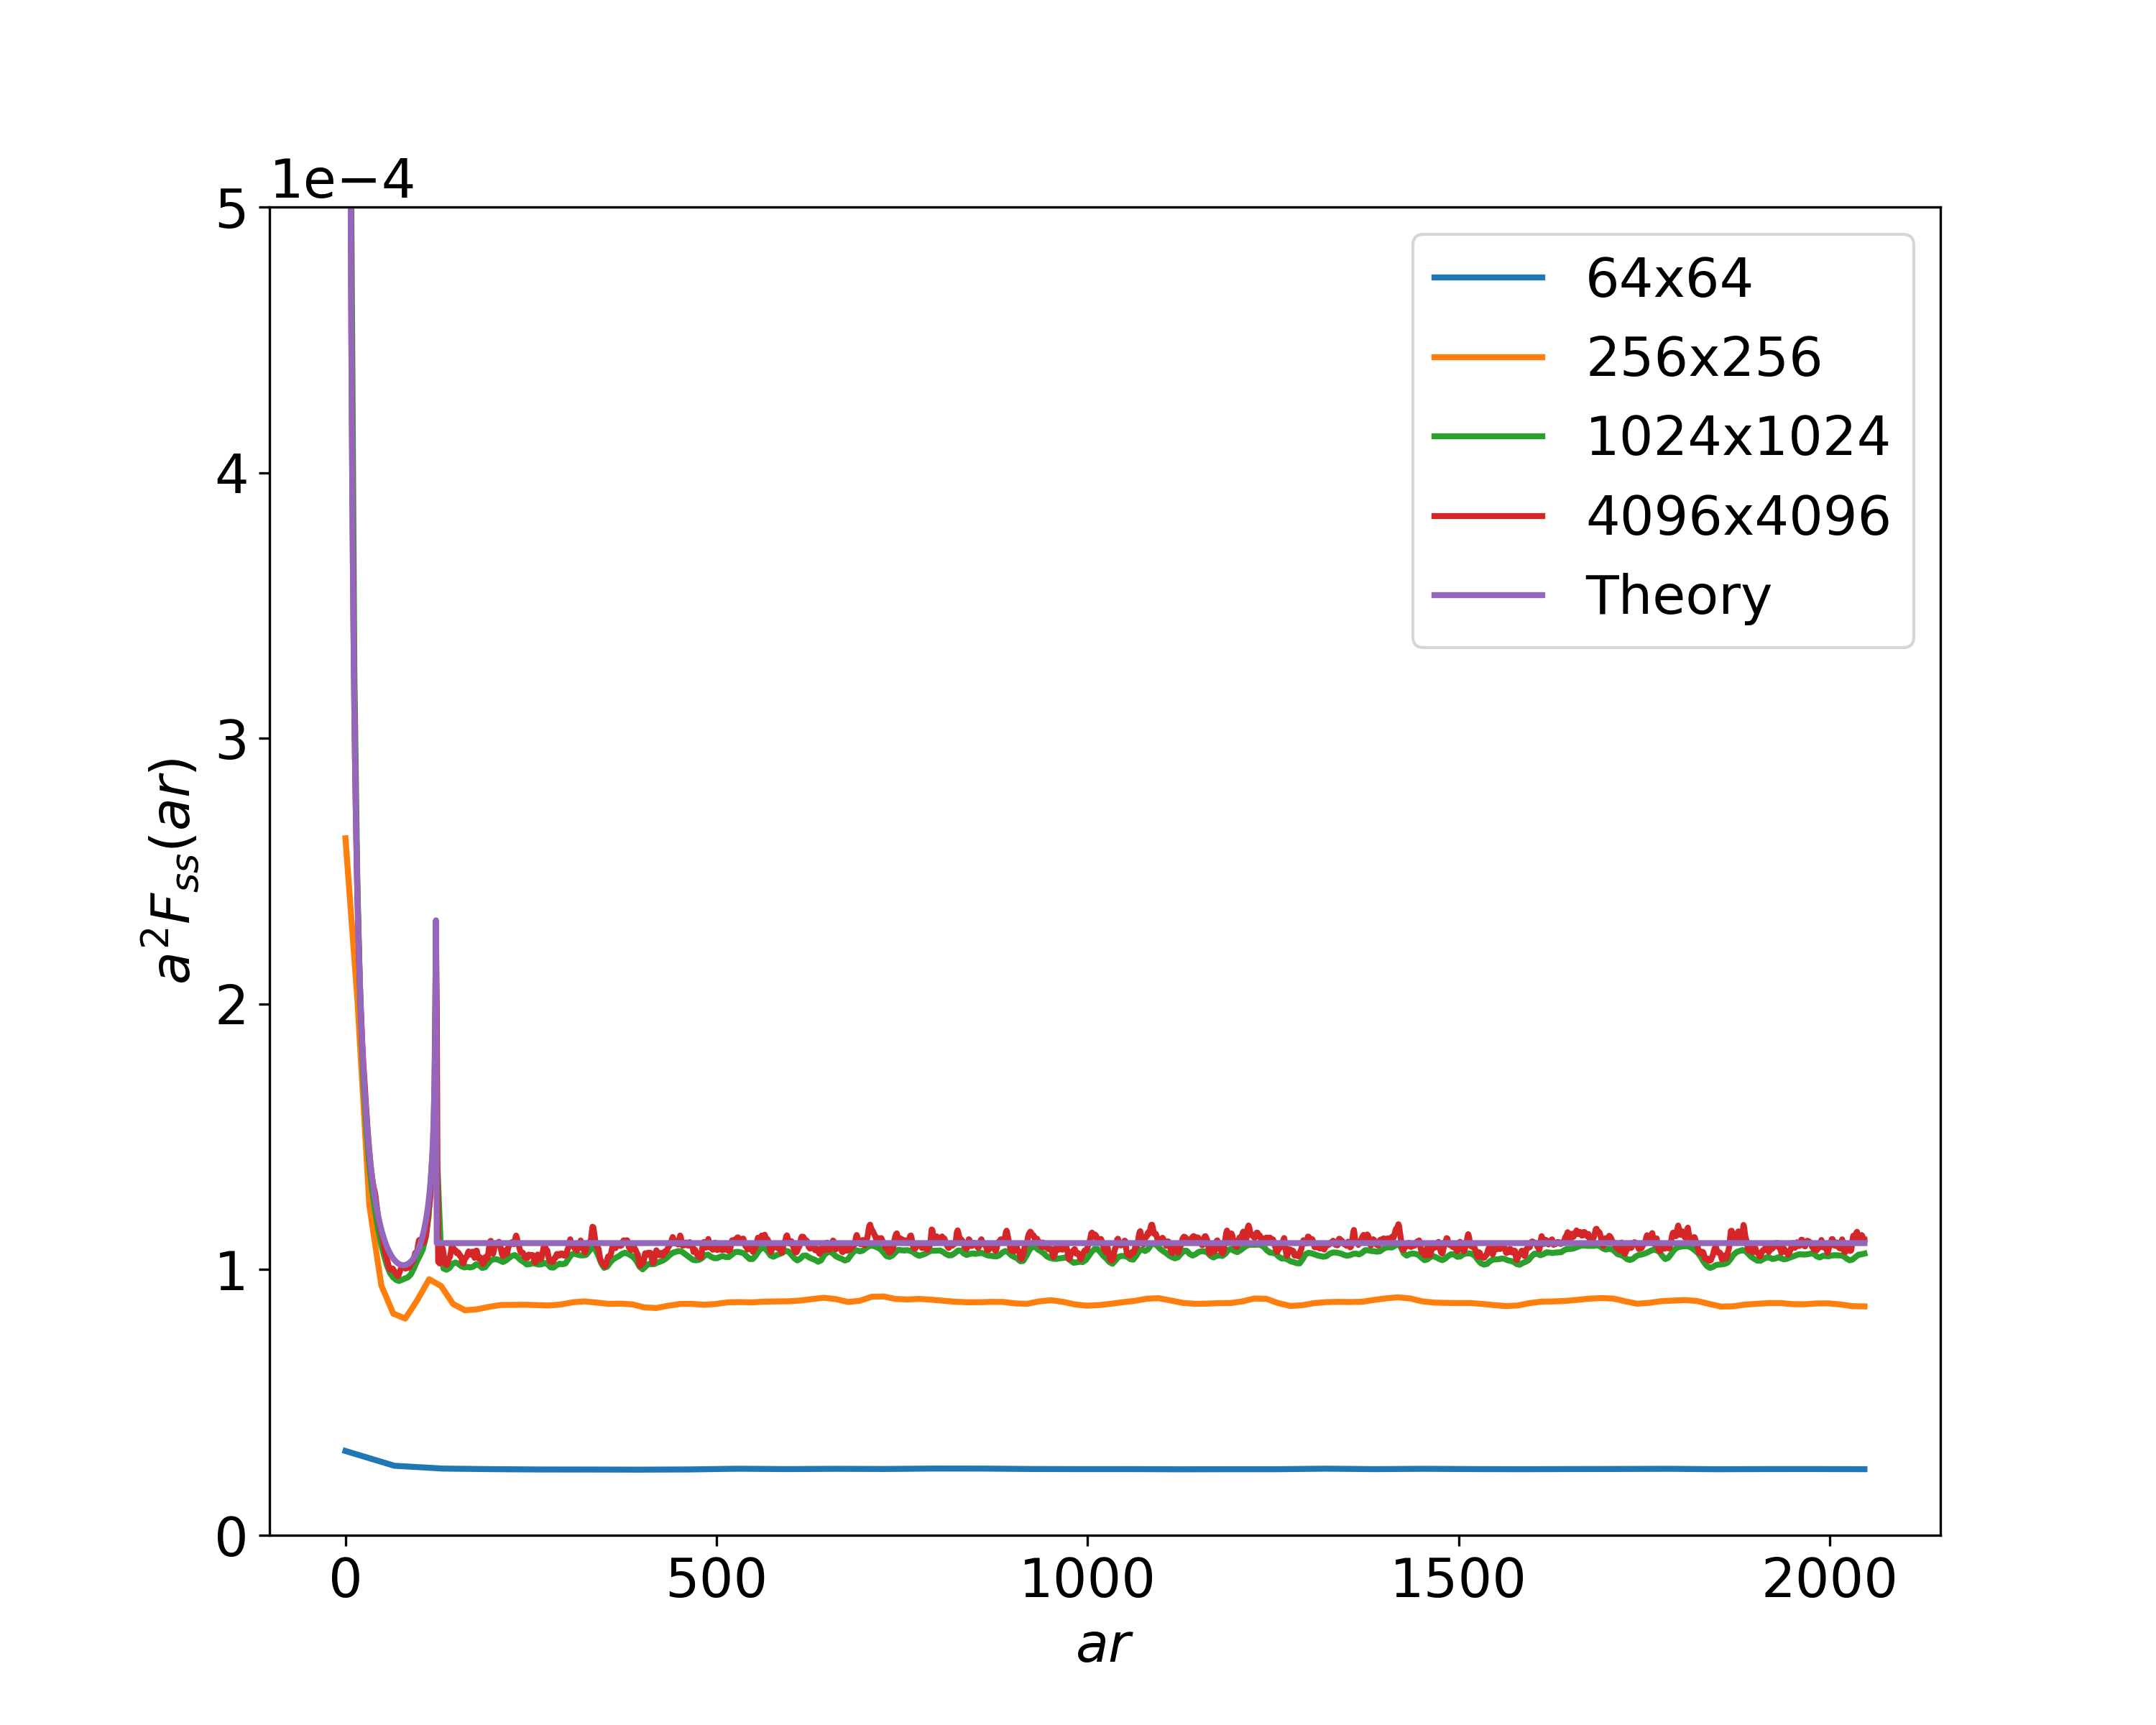
\includegraphics[width=0.475\linewidth]{images/plot-ss-balls.png}
    \label{fig:fss-scaling}}
  \hfill
  \subfigure[Surface-void]{
    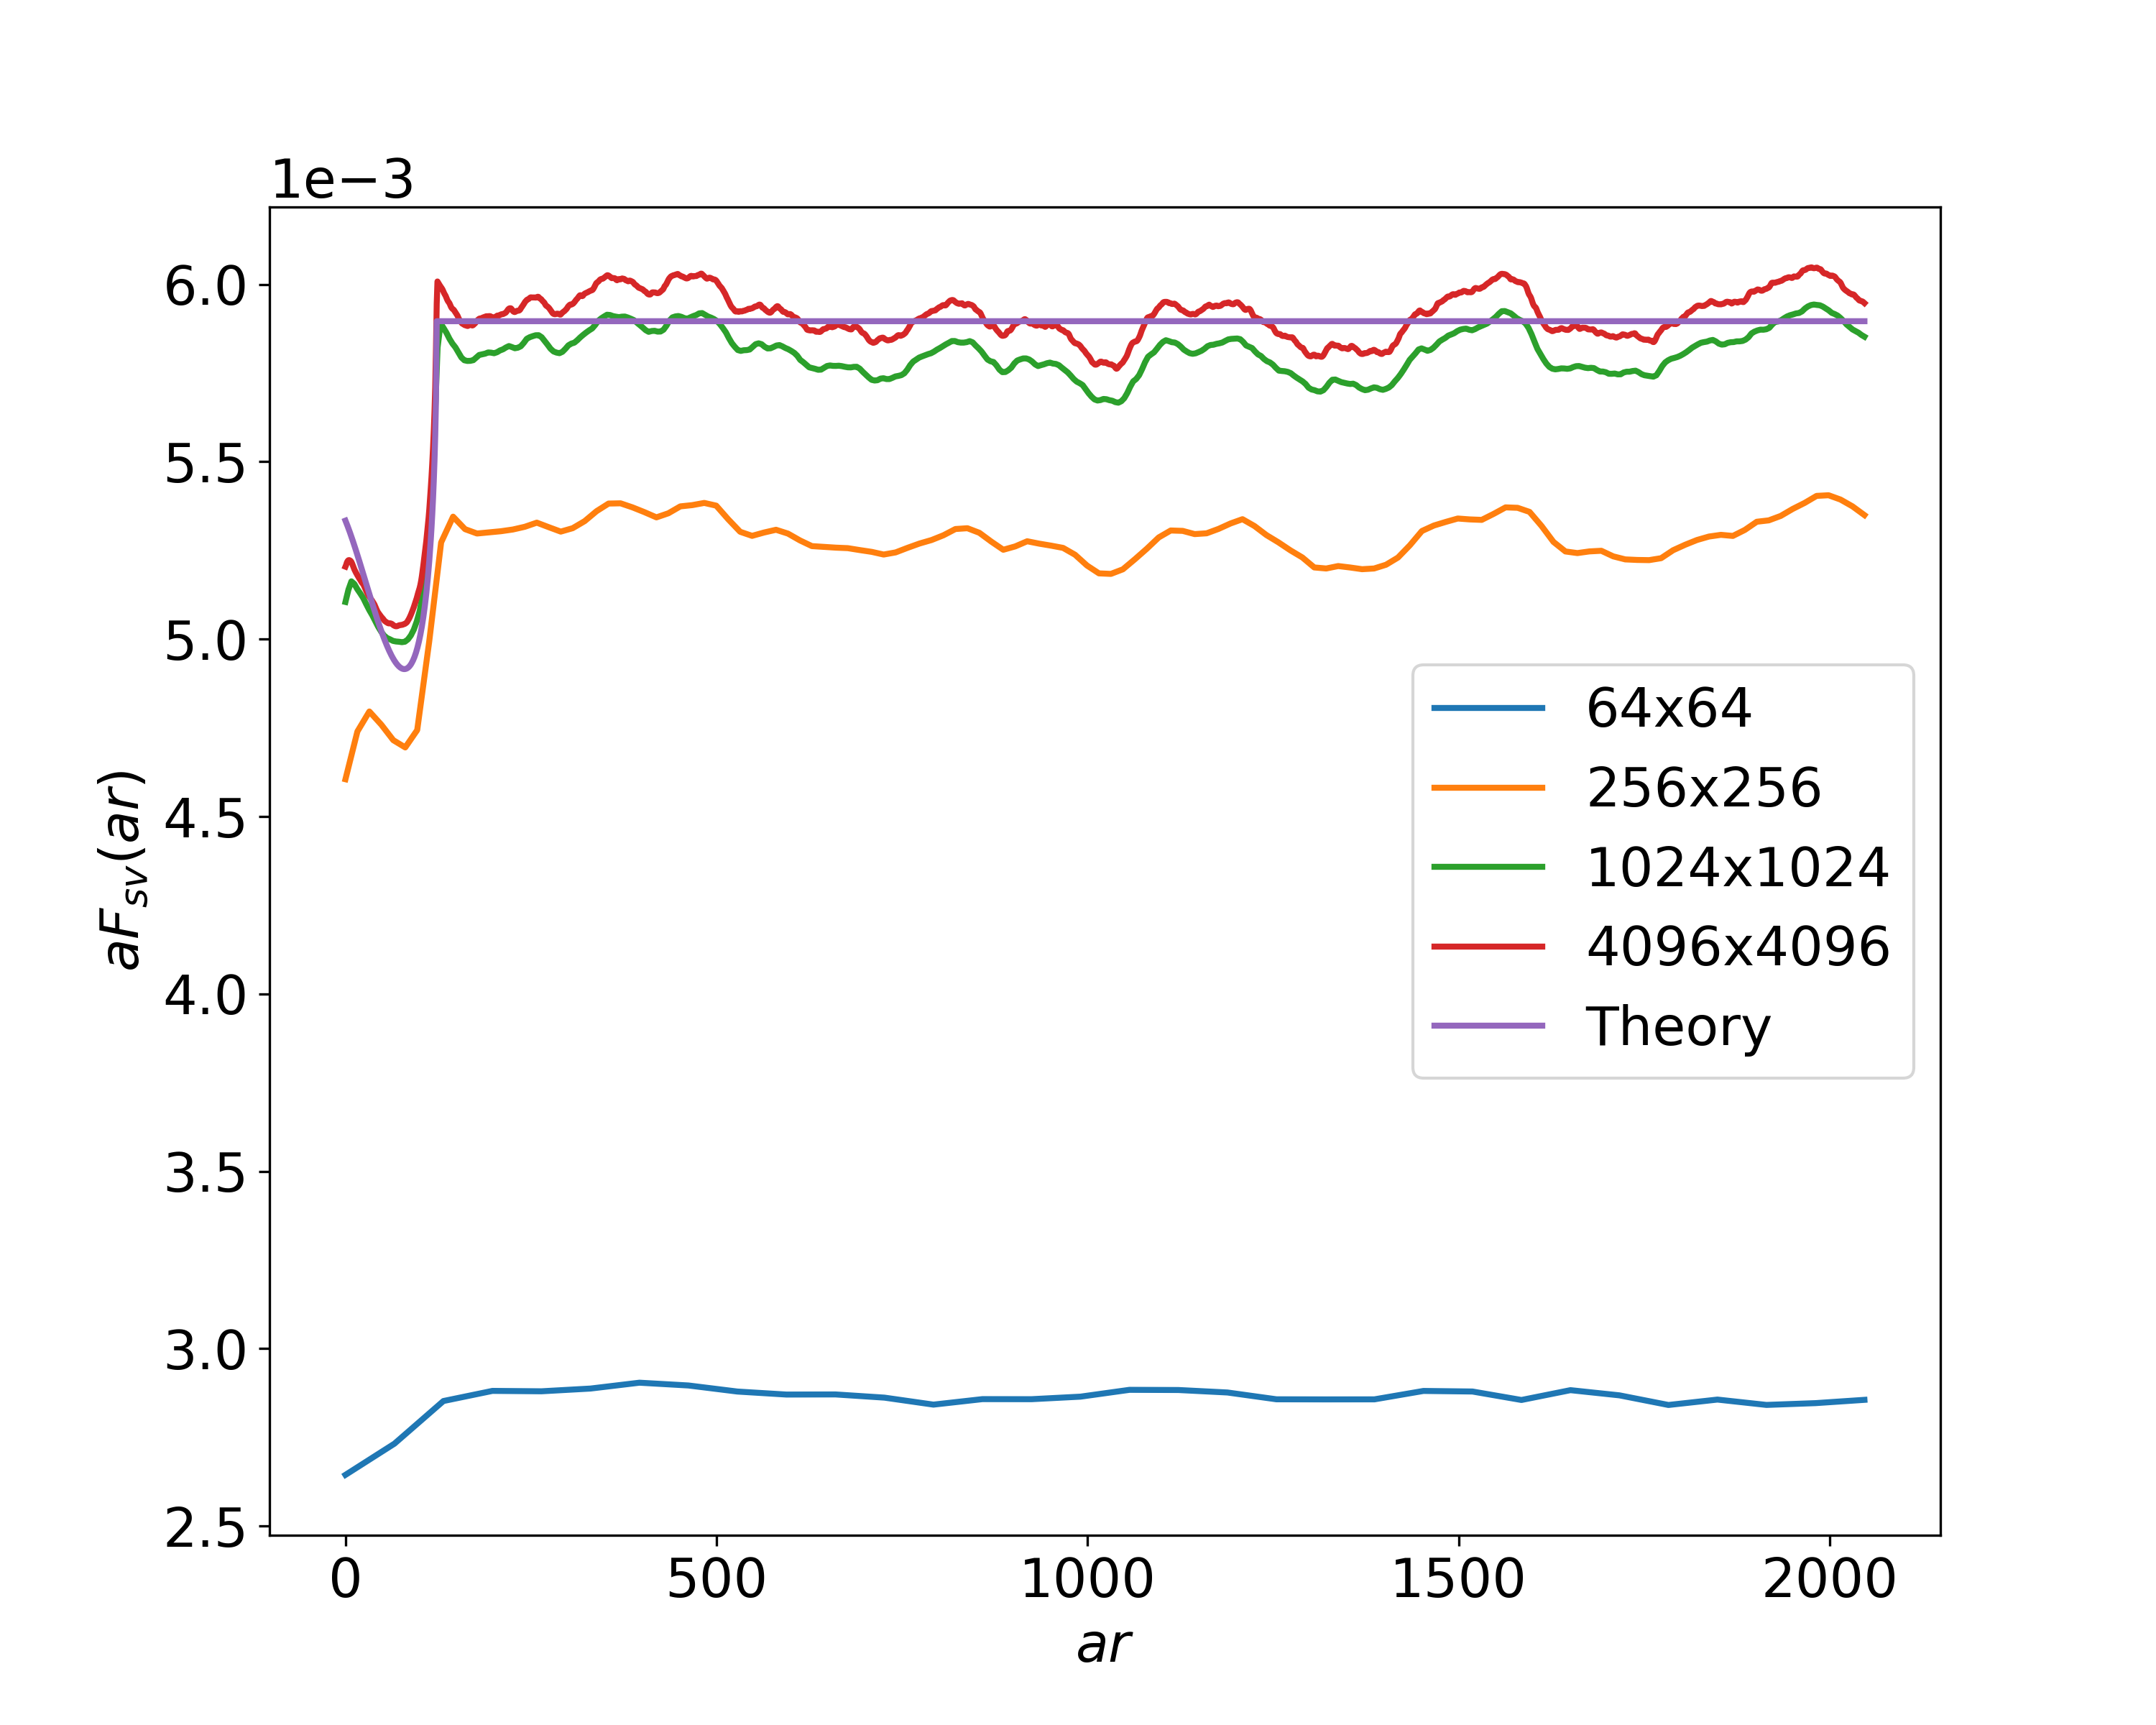
\includegraphics[width=0.475\linewidth]{images/plot-sv-balls.png}
    \label{fig:fsv-scaling}}
    \caption[]{The comparison of analytical and computed surface correlation
      functions for the Poisson disks for the original $4096 \times 4096$ pixels
      image. Computed CFs were obtained for different image resolutions as shown
      in the legend.}
    \label{fig:scaling}
\end{figure*}

We can observe two effects when downscaling the original image. The
first effect is that $F_{ss}(r)$ and $F_{sv}(r)$ for downscaled images lack in
detail (i.e. they are less ``noisy''). This can be easily explained by that the
interface between phases that becomes ``simpler'' when resolution decreases. The
second and much more important effect is that both correlation functions become
largely underestimated with the decline in resolution. This latter effect is in
general connected to the fact that the interface in digital images has
non-negligible thickness -- i.~e. the difference between real ``continuous''
interface versus ``digital'' interface (\cref{fig:scheme}). It is logical to
assume that with increasing spatial resolution the influence of this thickness
will diminish. This is exactly what we observe on \cref{fig:scaling} where
increasing disk discretization leads to convergence with analytical solution;
the accuracy of the computed CFs is almost perfect for discretization of about
12000 pixels for each disk. A natural question arises: ``Is there a criterion of
image quality (resolution) that allows to predict the quality of surface CFs
evaluation from digital images?''. Turns out there is a possibility to establish
such empirical criterion based on spectral analysis of input images and
\cref{sec:crit} provides necessary details.

Now consider a situation when an image is obtained by taking samples of a function
$f: \mathbb{R}^n \rightarrow \left\{0, 1\right\}$. The samples are taken from a
regular grid which covers the range $[0, 1]^n$  with interval $\Delta$ between
samples. The resulting image has then $1/\Delta + 1$ pixels in each
dimension. An example of $f$ is a thresholded value noise function, and an
example of image generated by sampling this function is on \cref{fig:noise}.

\begin{figure}[ht]
  \centering
  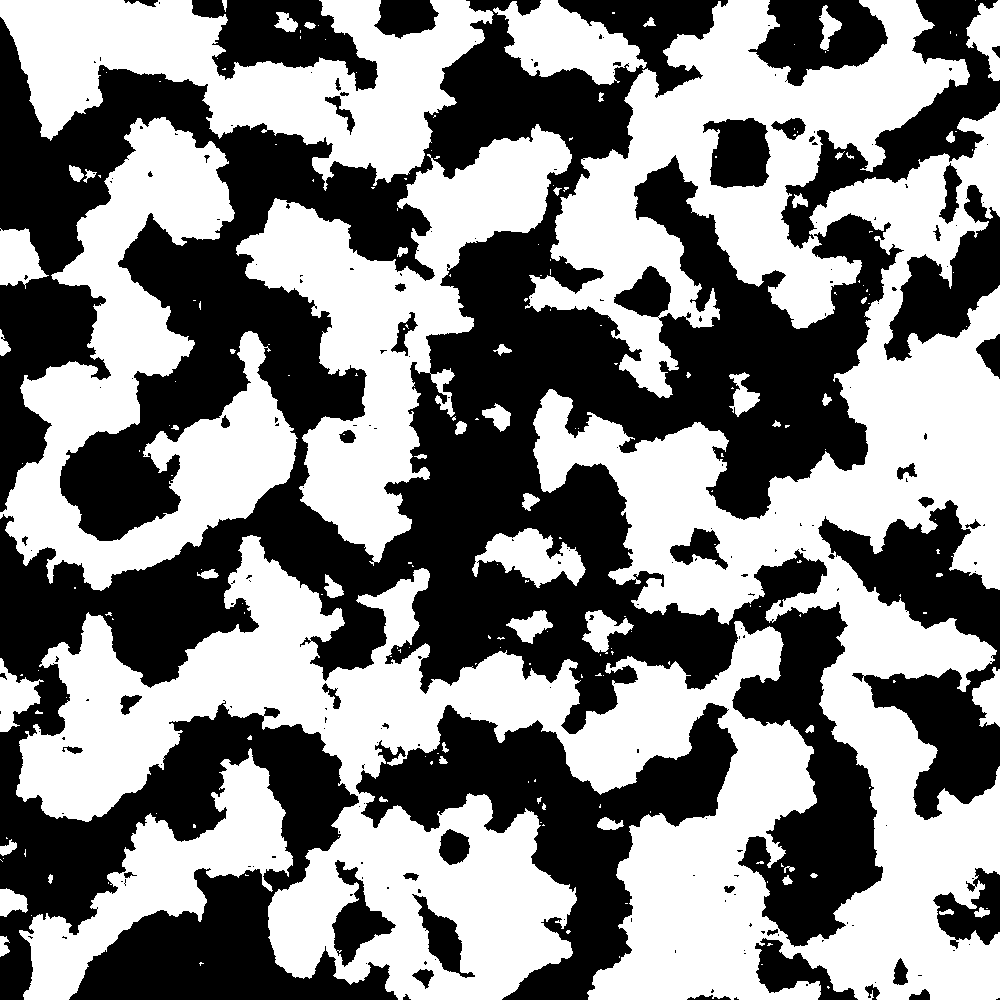
\includegraphics[width=0.9\linewidth]{images/noise.png}
  \caption[]{Example of thresholded value noise used for study of sampling
    effects.}
  \label{fig:noise}
\end{figure}

If we calculate surface-surface and surface-void correlation functions for these
images and scale them as described above, we will converge to some ``true''
correlation functions for continuous function $f$.

\begin{figure*}[ht]
  \centering
  \subfigure[Surface-surface]{
    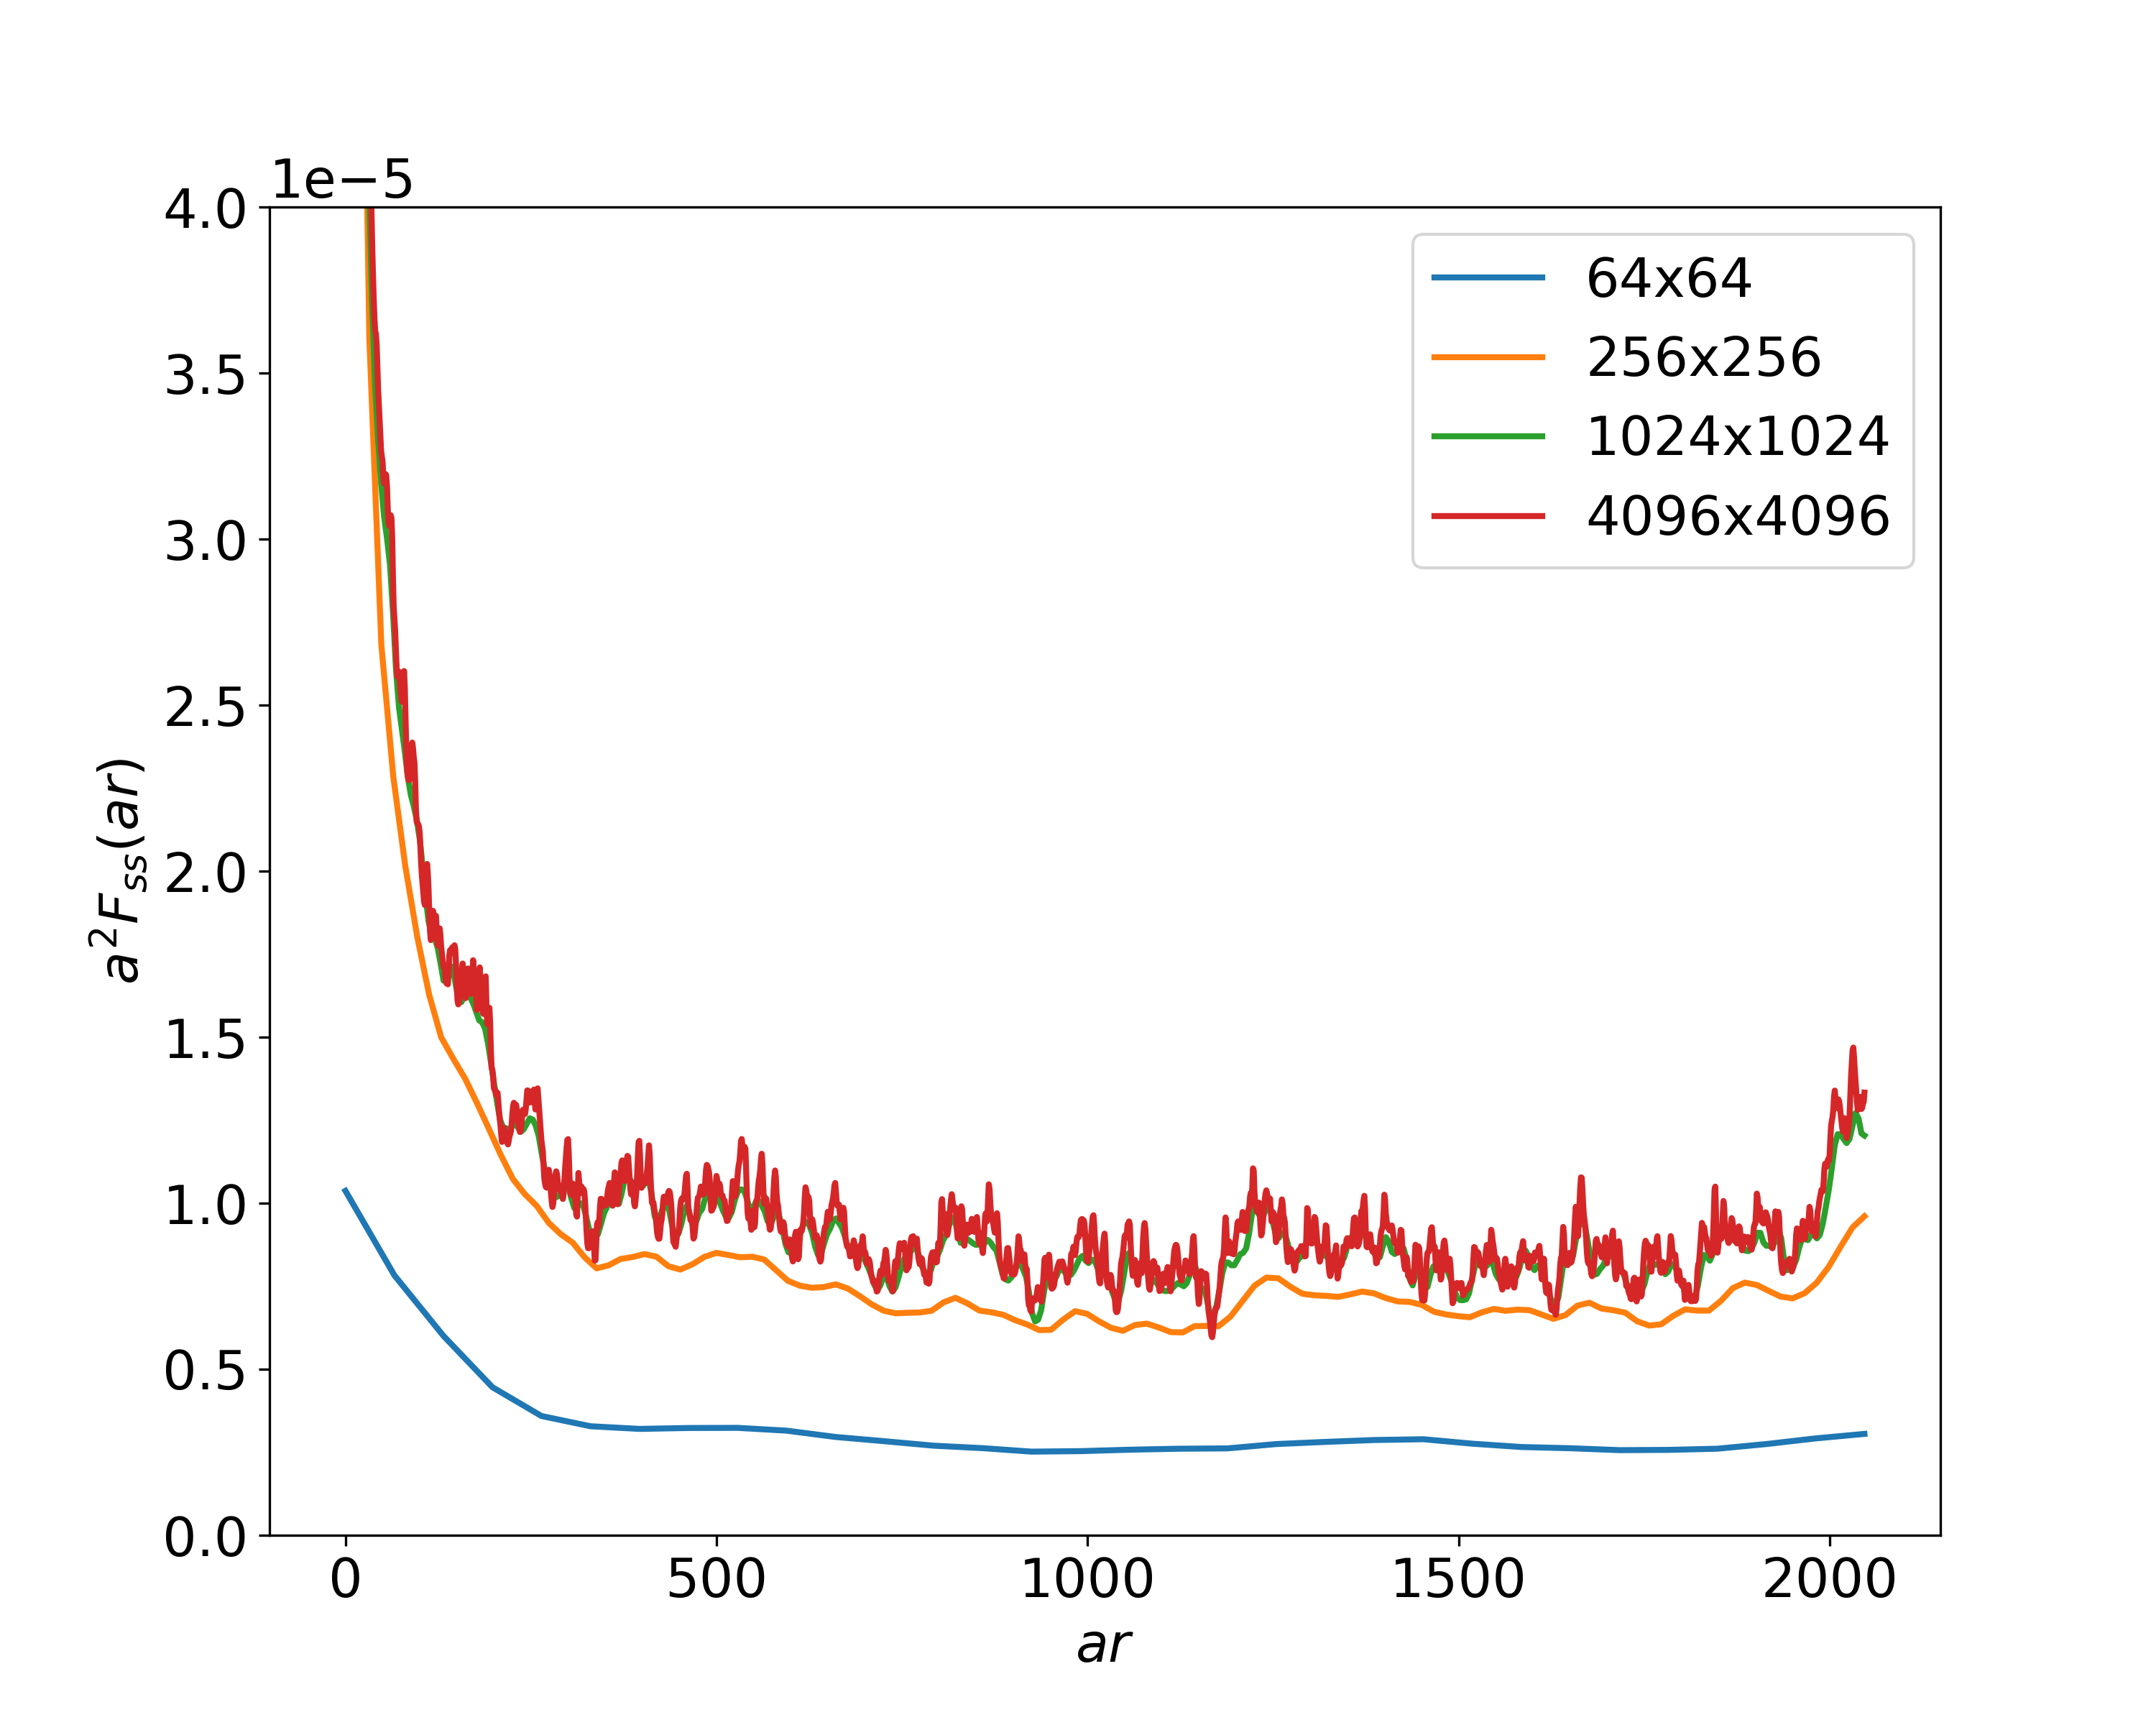
\includegraphics[width=0.475\linewidth]{images/plot-ss-noise.png}
    \label{fig:fss-scaling-noise}}
  \hfill
  \subfigure[Surface-void]{
    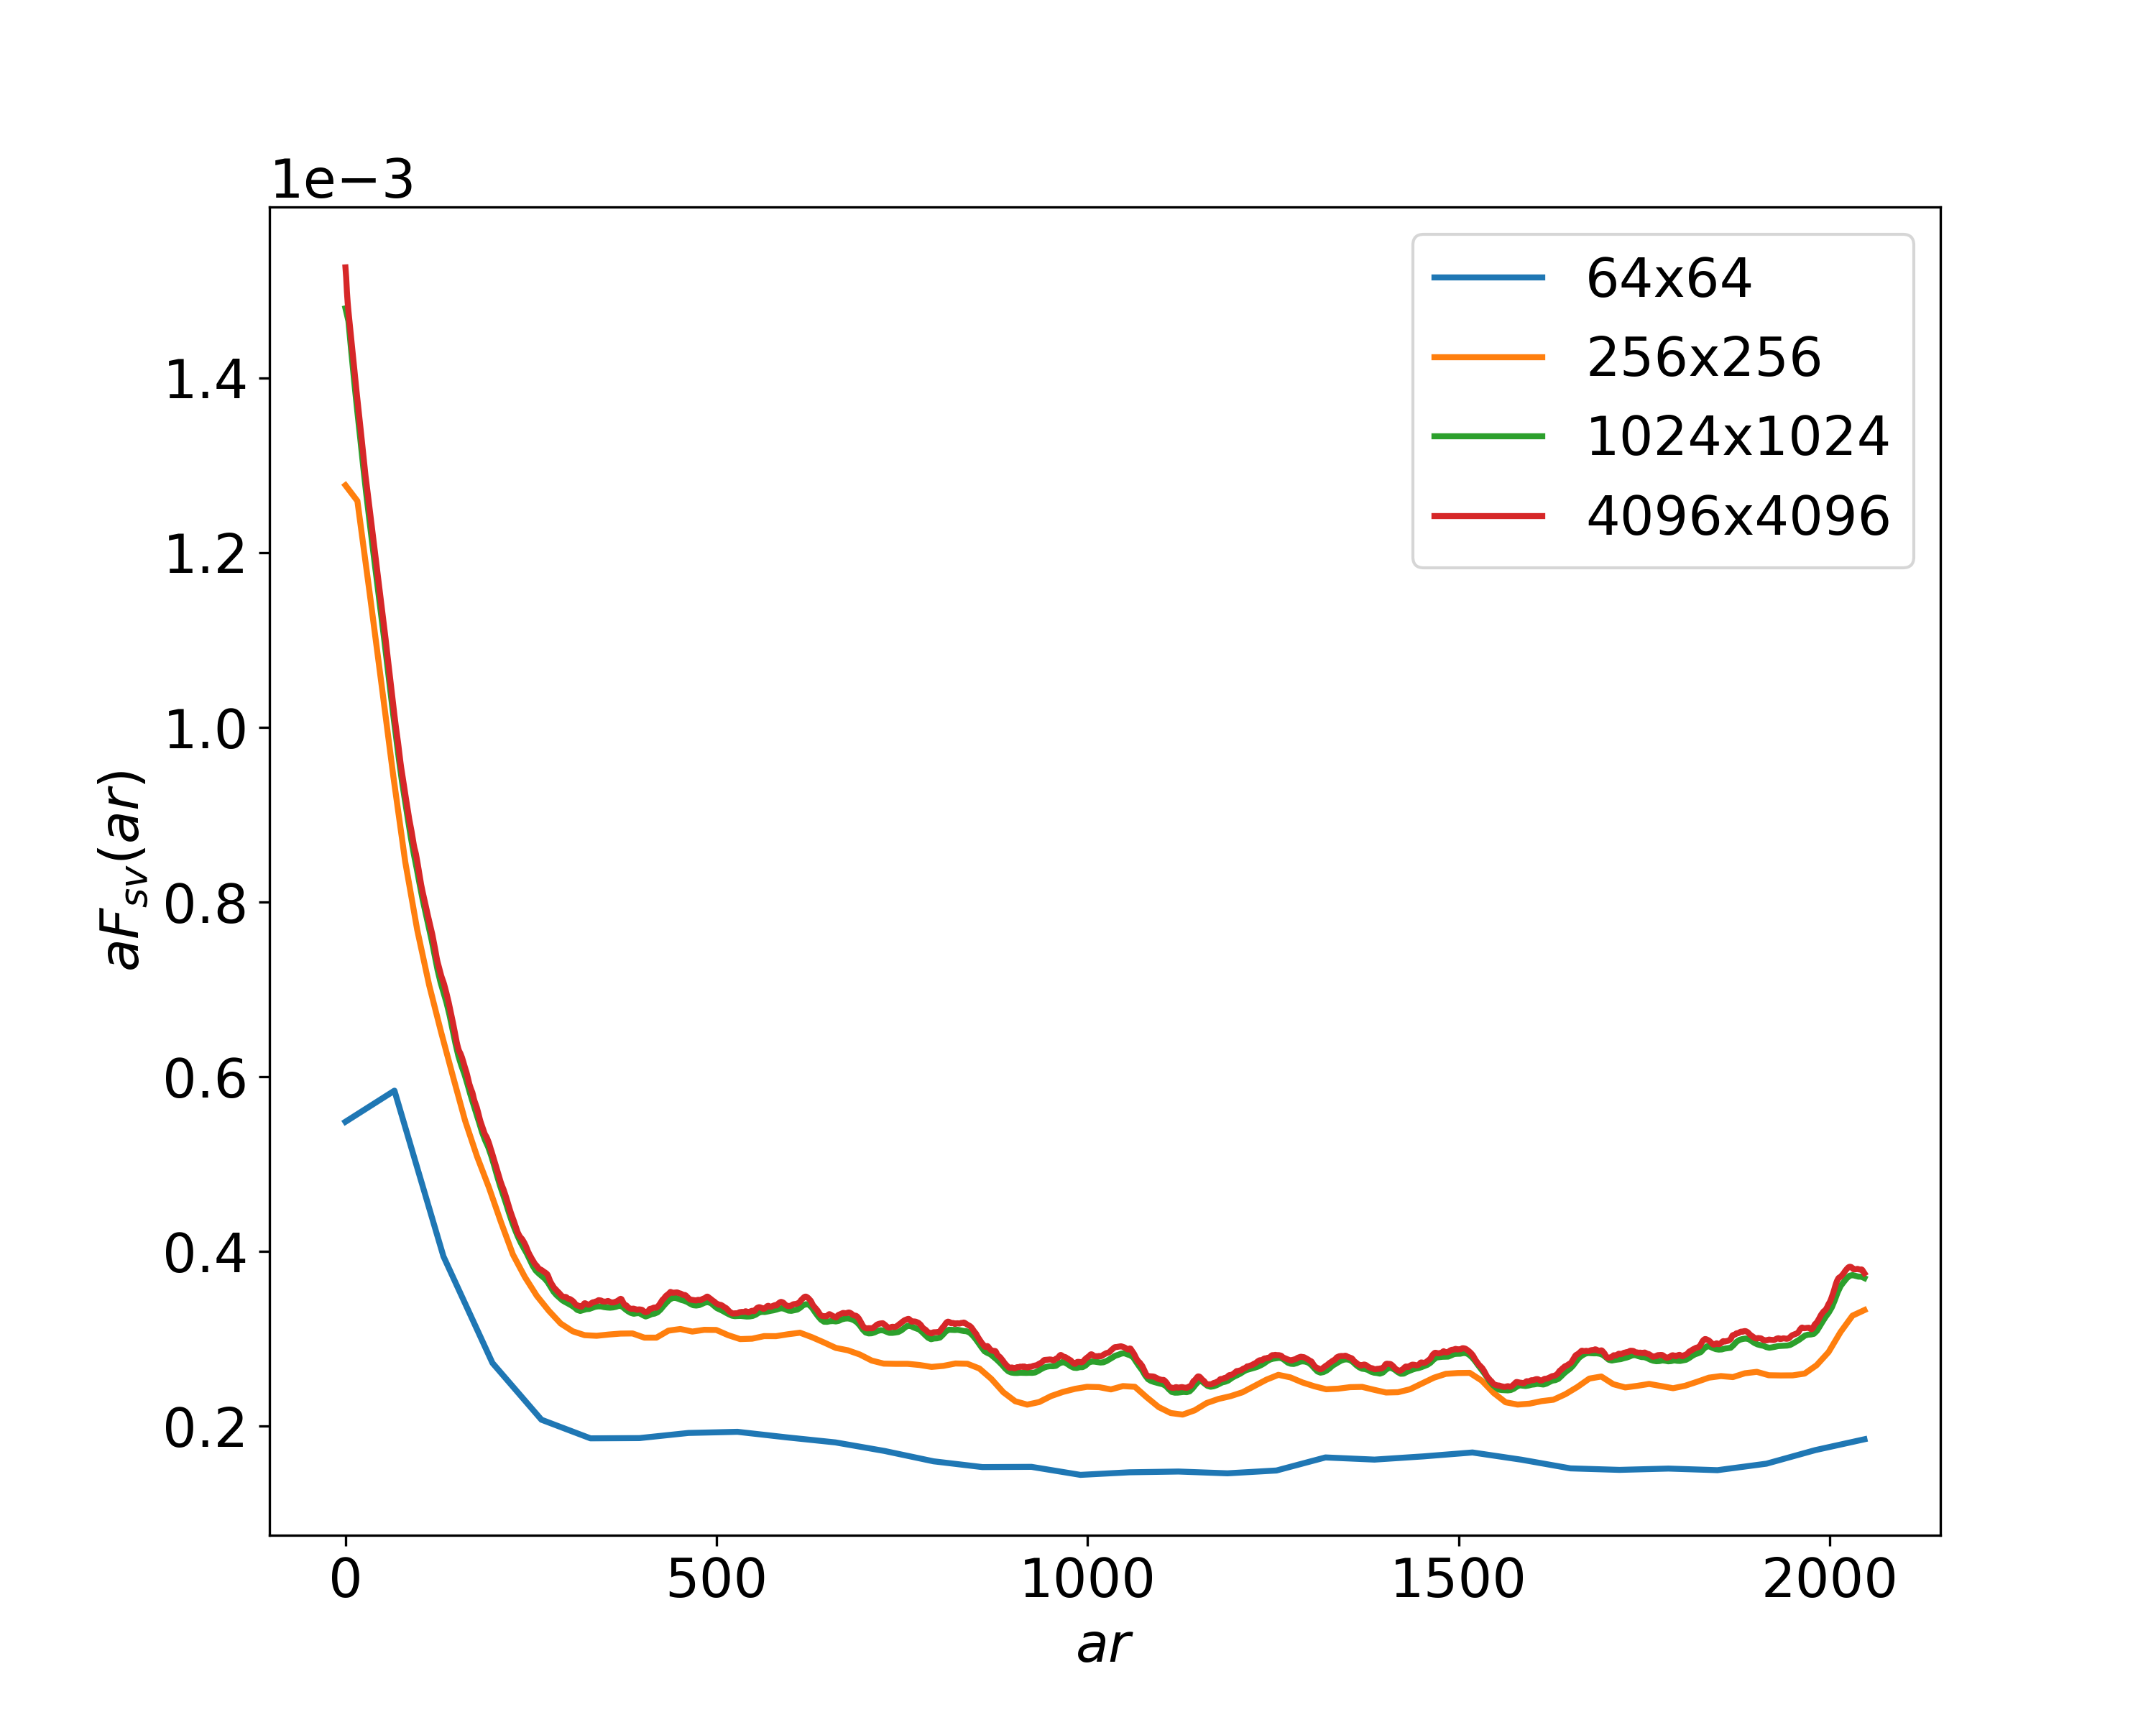
\includegraphics[width=0.475\linewidth]{images/plot-sv-noise.png}
    \label{fig:fsv-scaling-noise}}
    \caption[]{Surface-surface and surface-void correlation functions for
      thresholded value noise function sampled with different resolutions.}
    \label{fig:scaling-noise}
\end{figure*}

\subsection{The choice of filter’s kernel to extract the interface (gradient)}
There are many different kernels to evaluate gradients, but the Sobel kernel
performed slightly better \cref{fig:wtf2} compared to majority of other kernels
we have explored: Ando, Scharr, Bickley, and Prewitt filters. Only the Ando’s
filter with size of $5 \times 5$ \cite{ando_2000} outperformed the Sobel filter
in terms of error minimization for 2D disks surface CFs
computation. Nonetheless, we chose Sobel filter due to its simplicity, faster
computations and robust implementation of the 3D kernel in all major libraries
(where Ando is only a 2D filter). Gauss filter is not improving \cref{fig:wtf3}.

\subsection{Criteria for accurate evaluation of surface CFs from discrete images}
\label{sec:crit}
Let us define one-dimensional forward ($F$) and inverse ($F^{-1}$) Fourier
transforms as:
\begin{align}
  \hat{f}(z) &= F[f](z) = \frac{1}{\sqrt{2\pi}}\int_{-\infty}^{\infty} f(x)
  e^{-i\pi xz} dx \label{eq:fourier-forward} \\
  f(x) &= F^{-1}[\hat{f}](z) = \frac{1}{\sqrt{2\pi}}\int_{-\infty}^{\infty} \hat{f}(z)
  e^{i\pi xz} dz \label{eq:fourier-backward}
\end{align}

Here $f(x)$ and $\hat{f}(z)$ can be thought of as representations of a signal in
the time domain and the frequency domain, respectively. Both equations
\cref{eq:fourier-forward} and \cref{eq:fourier-backward} preserve norm on $L_2$:
$(f, f) = (\hat{f}, \hat{f})$. It is said that Fourier transform preserves
``energy'' of the signal. According to Riemann-Lebesgue lemma \cite{bookHilb}
energy of any signal ``concentrates'' around low frequencies. A measure of how
much energy concentrated in low frequencies (for some definition of low
frequencies) is a key to the understanding of the problem of correctness of our
method. The Shannon sampling theorem \cite{bookHilb} states that it is possible
to reconstruct a band-limited signal $f(x)$ whose frequencies lie in the range
$[0, f]$ from a sequence of samples $\left\{f_n\right\}$ if the sampling rate is
no less than $2f$. We introduce a parameter $C_a$:
\begin{align*}
  f_0(x) &= f(x) - \langle f(x) \rangle \\
  C_a &= \frac{\int_{-a\omega}^{a\omega} |\hat{f_0}(z)|^2 dz}{\int_{-\omega}^{\omega} |\hat{f_0}(z)|^2 dz}
\end{align*}
where $\omega = 2\pi f$ and $\langle f(x) \rangle$ is the mean value of $f(x)$
over its domain. The criterion for correctness is then:
\begin{equation*}
  C_a > 1 - \xi
\end{equation*}
for some $a$ and $\xi$. This criterion tells us exactly how much energy in
$f_0(x)$ is concentrated in a low frequency range $[0, af]$ compared to the
whole range $[0, f]$. In our work we propose $a = 0.5$ and $\xi = 0.07$ as
a strict criterion which is based on results of section
\cref{sec:comparison}. For the images of Poisson disks from \cref{fig:scaling}
their discretizations and $C_{0.5}$ are shown in \cref{fig:disks-res}. We
immediately observe that the images on top (with resolution $4096 \times 4096$
and $1024 \times 1024$) have surface CFs very close to analytical solution and
satisfy our  $C_{0.5}$ criterion perfectly. The other two downscaled images fail
to satisfy the criterion. As we can see in conjunction from \cref{fig:scaling}
and \cref{fig:disks-res} the criterion correctly selects images which are
suitable for calculation of the correlation functions using Method2 and
Method3. The criterion $C_{0.5}$ decays fast with the decline in image
resolution as shown in \cref{fig:crit-plot}.

\begin{figure}[ht]
  \centering
  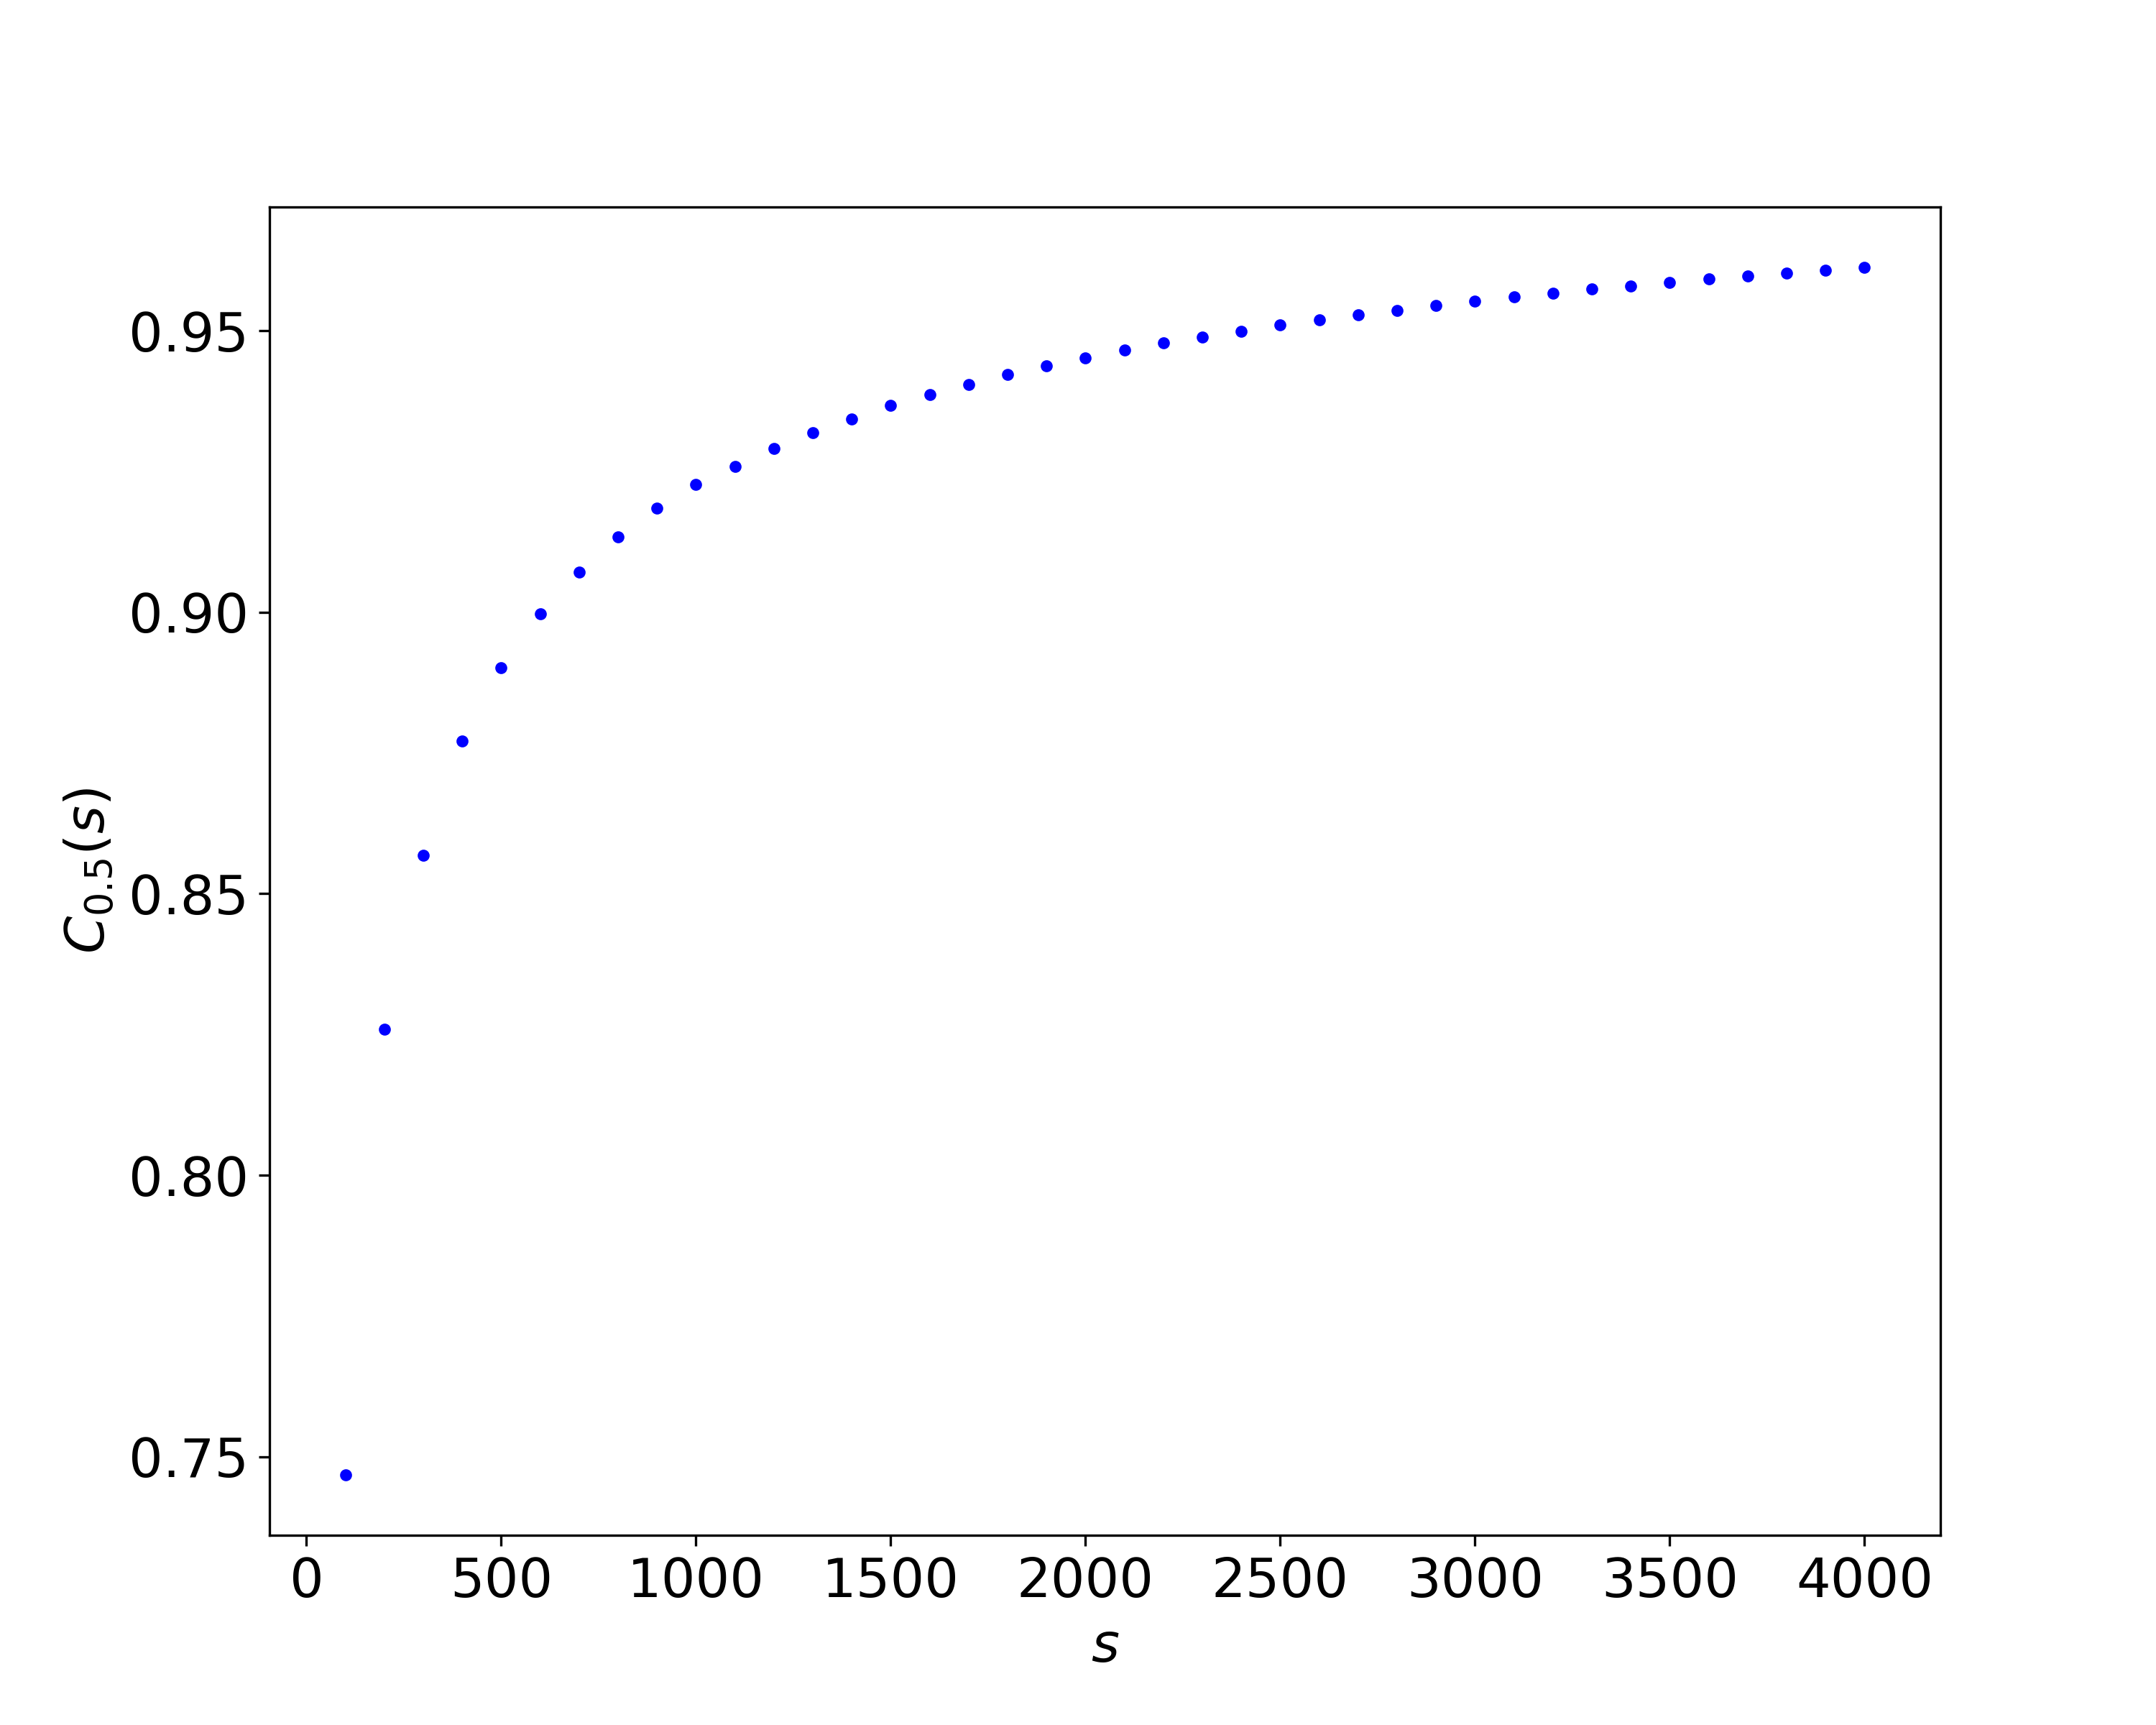
\includegraphics[width=0.9\linewidth]{images/plot-criterion.png}
  \caption[]{The decay of criterion $C_{0.5}$ as a function of the size $s$ of
    the downscaled image.}
  \label{fig:crit-plot}
\end{figure}

\begin{figure*}[t]
  \centering
  \subfigure[Resolution $4096 \times 4096$, disk radius 61.44 pixels, $C_{0.5} = 0.9593$]{
    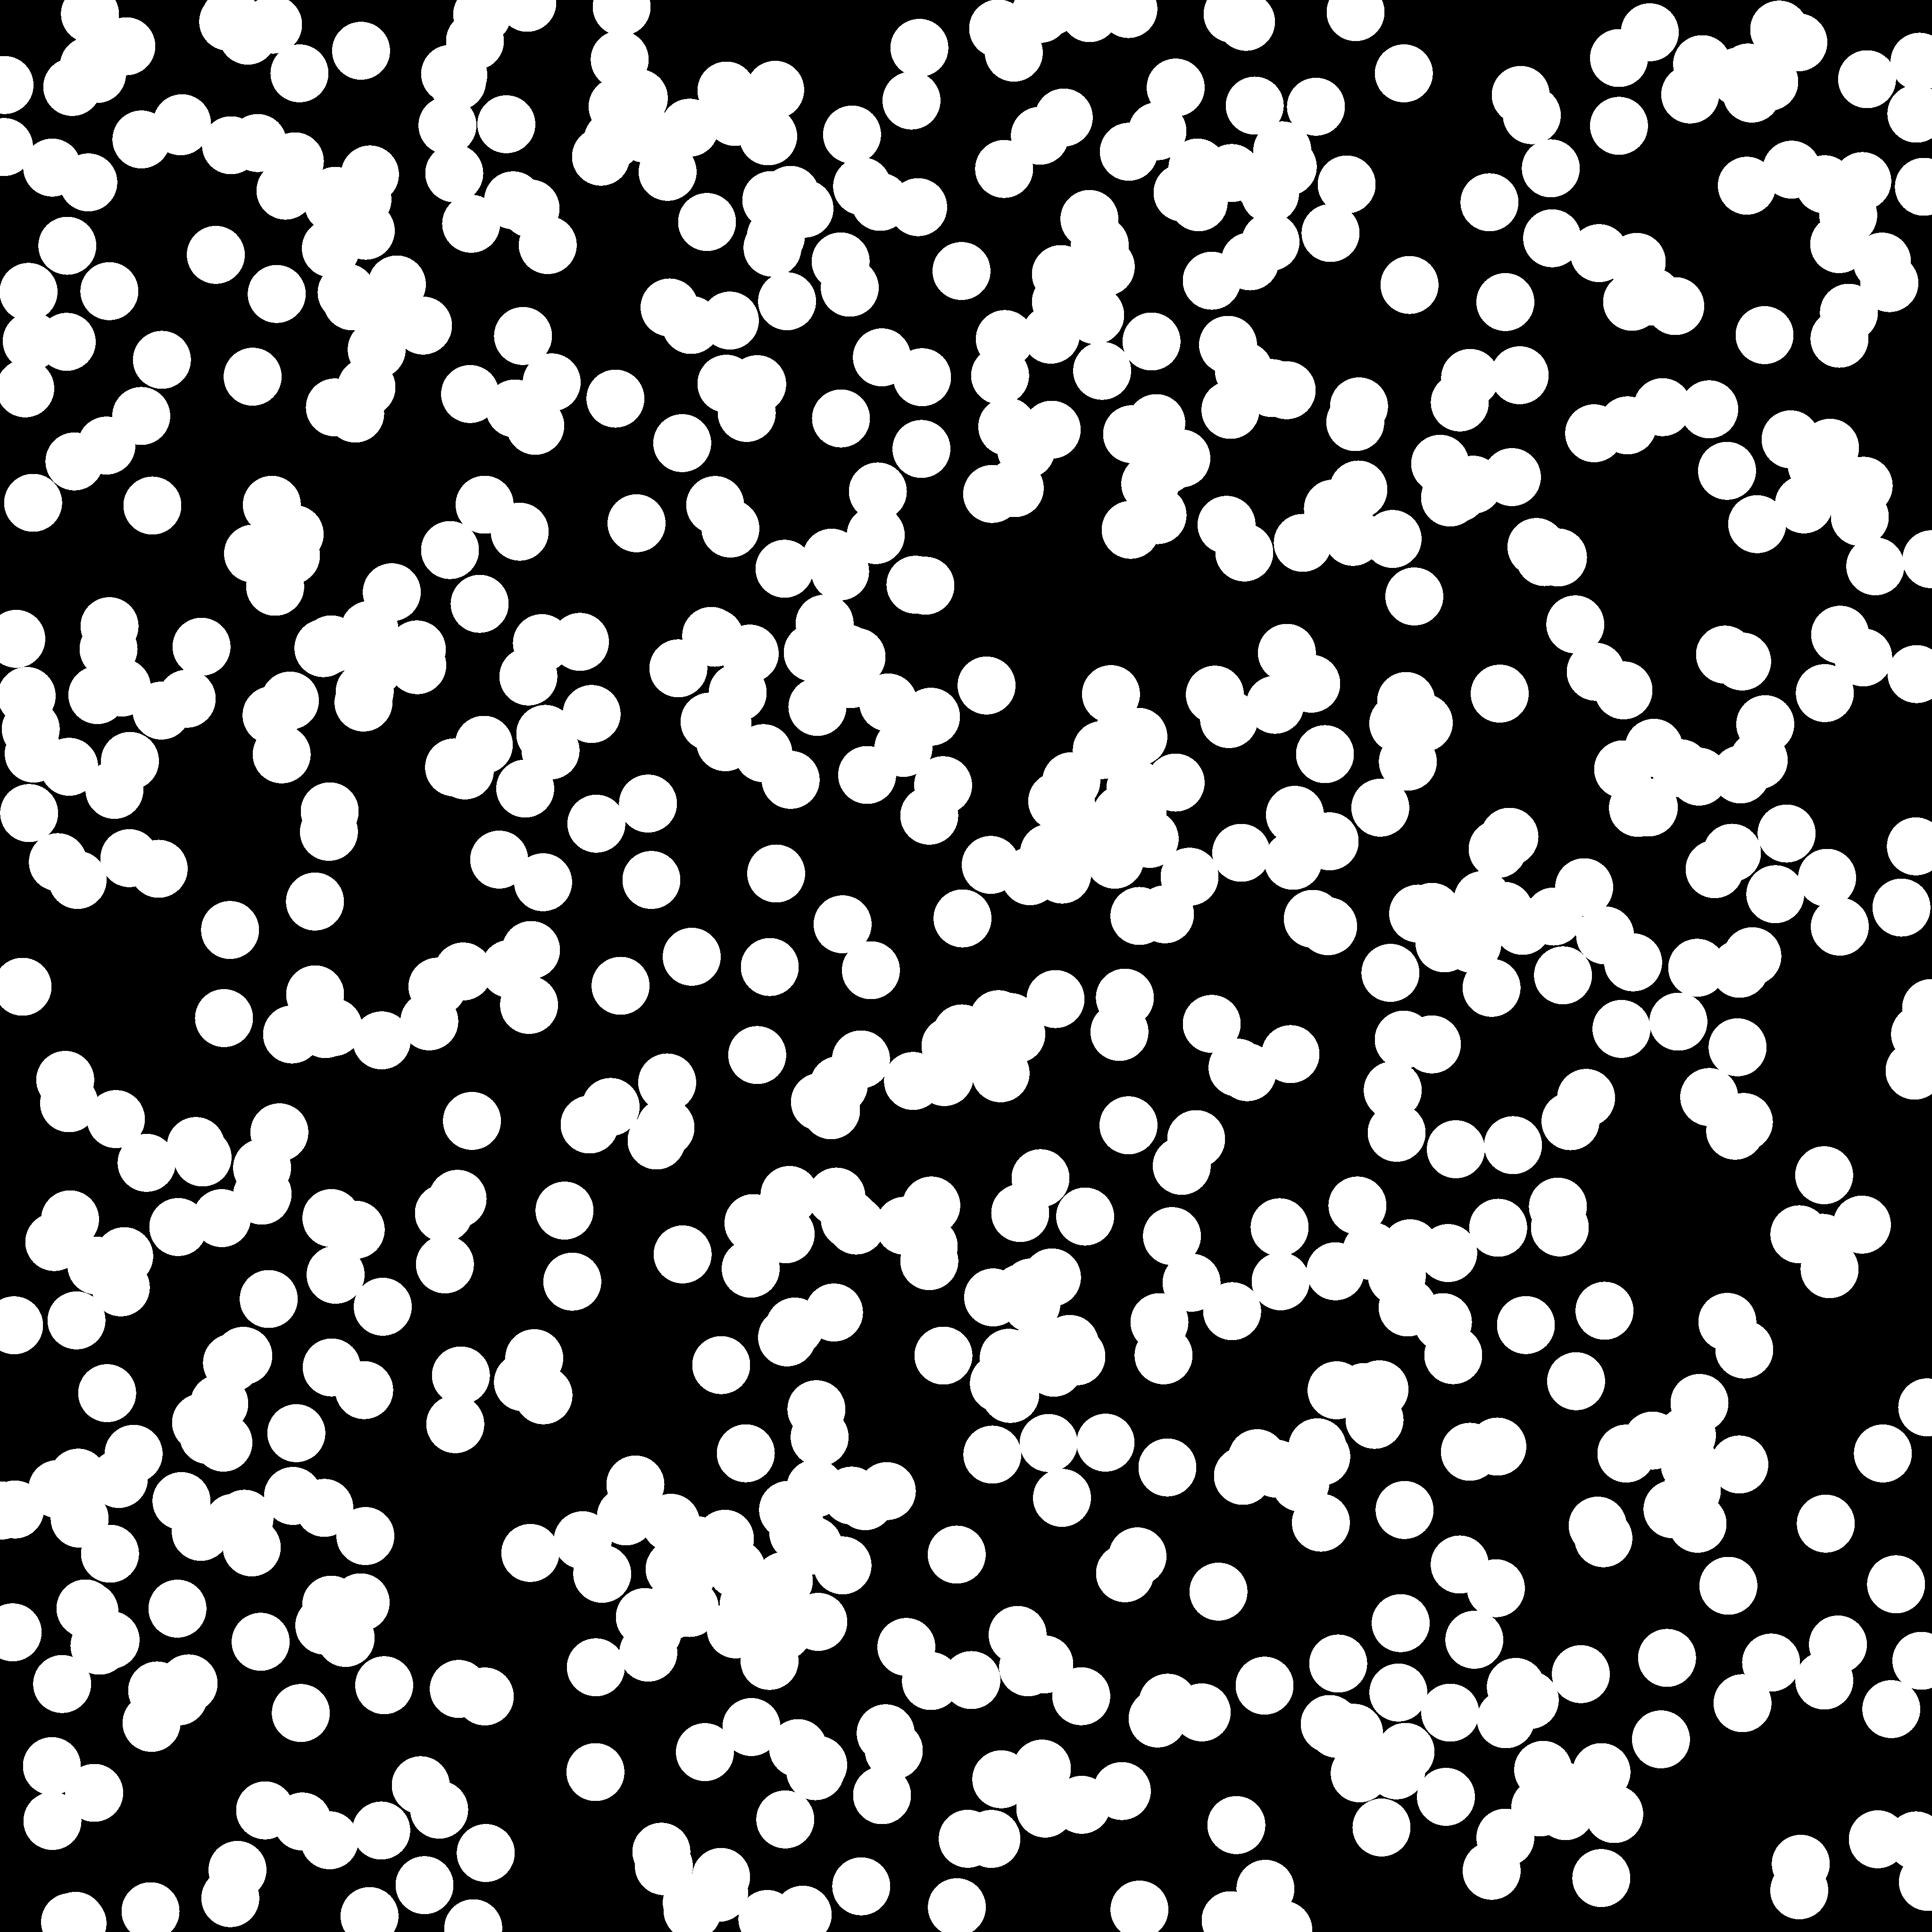
\includegraphics[width=0.475\linewidth]{images/disks-0015-5e-5-4096.png}
    \label{fig:disks-4096}}
  \hfill
  \subfigure[Resolution $1024 \times 1024$, disk radius 15.36 pixels, $C_{0.5} = 0.9185$]{
    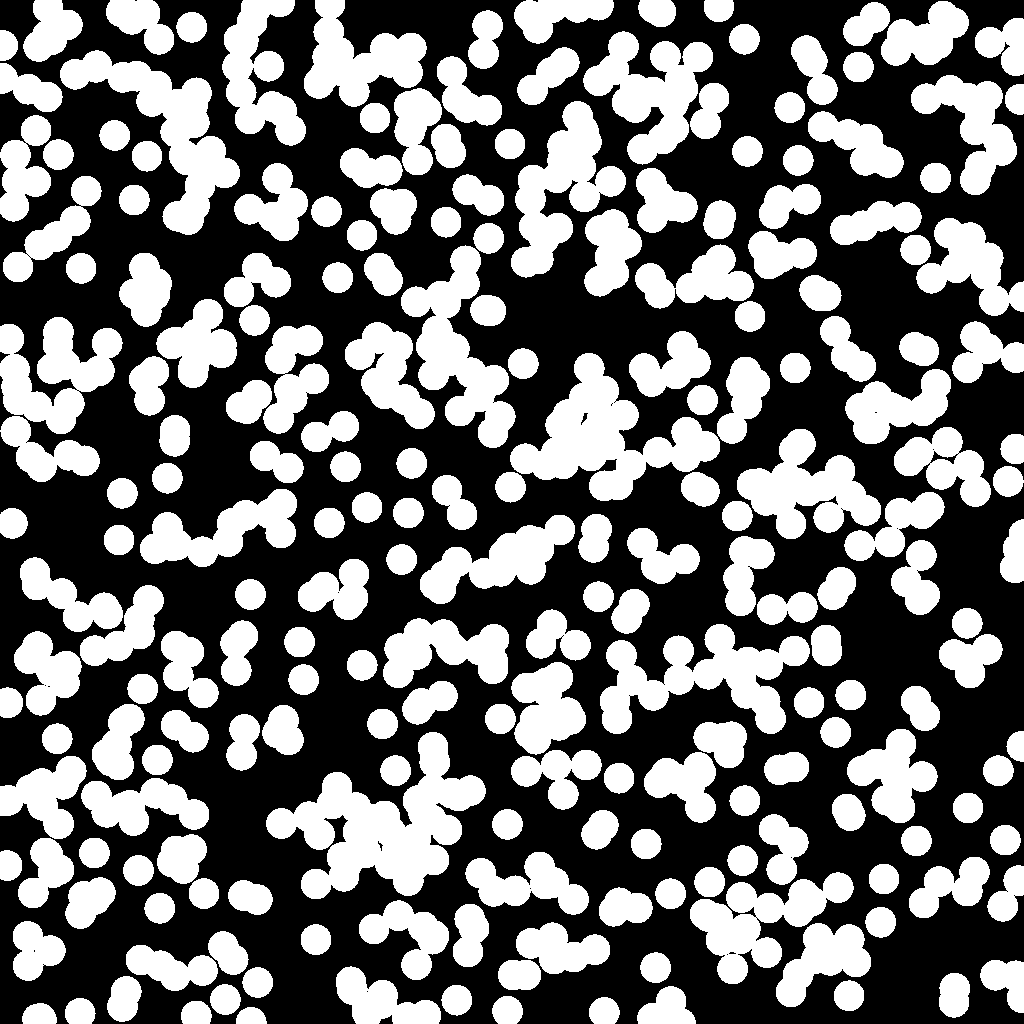
\includegraphics[width=0.475\linewidth]{images/disks-0015-5e-5-1024.png}
    \label{fig:disks-1024}}
  \vskip\baselineskip
  \subfigure[Resolution $256 \times 256$, disk radius 3.84 pixels, $C_{0.5} = 0.8356$]{
    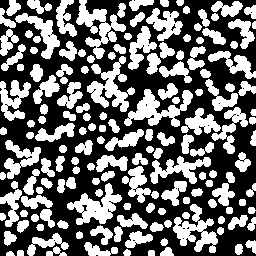
\includegraphics[width=0.475\linewidth]{images/disks-0015-5e-5-256.png}
    \label{fig:disks-256}}
  \hfill
  \subfigure[Resolution $64 \times 64$, disk radius 0.96 pixels, $C_{0.5} = 0.6549$]{
    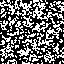
\includegraphics[width=0.475\linewidth]{images/disks-0015-5e-5-64.png}
    \label{fig:disks-64}}
  \caption[]{The influence of imaging resolution on the quality of surface
    correlation functions computations (as shown in \cref{fig:scaling}) based on
    the criterion $C_{0.5}$.}
  \label{fig:disks-res}
\end{figure*}

\subsection{Application to binary images of porous media}
\label{sec:application}
After the verification of our computational approach based on analytical
solution and establishing the criterion $C_{0.5}$ we now have enough tools to
evaluate surface CFs for different porous media images, including real XCT and
SEM images.

For demonstration purposes, we computed correlation functions for three
sandstone and three carbonate samples with dimensions
$500 \times 500 \times 500$ (\cref{fig:real-data}) all of which satisfy our
$C_{0.5}$ criterion. The result can be seen on \cref{fig:real-data-plots}.

There are examples of bad images which do not pass our criterion on
\cref{fig:real-bad}.

\begin{figure*}[t]
  \centering
  \subfigure[Sandstone 1, $C_{0.5} = 0.938$]{
    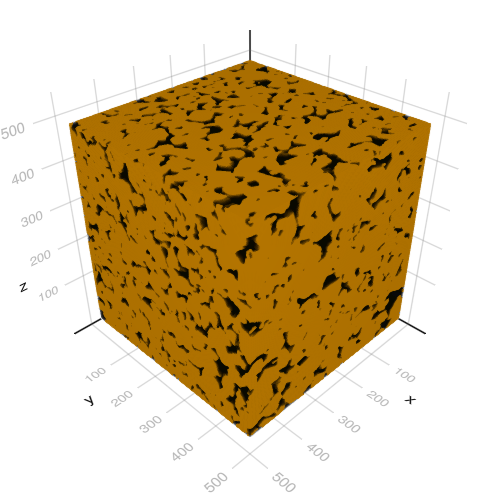
\includegraphics[width=0.3\linewidth]{images/sandstone1.png}
    \label{fig:sandstone1}}
  \hfill
  \subfigure[Sandstone 2, $C_{0.5} = 0.937$]{
    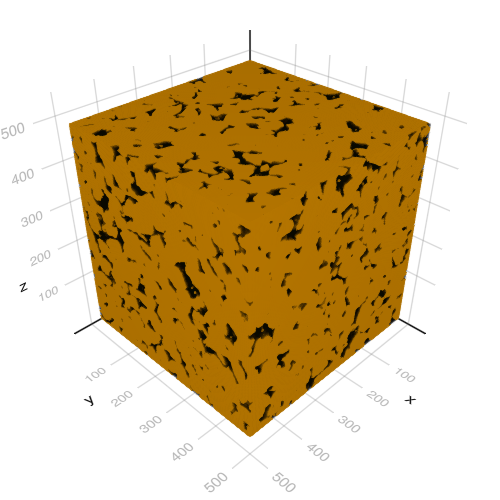
\includegraphics[width=0.3\linewidth]{images/sandstone2.png}
    \label{fig:sandstone2}}
  \hfill
  \subfigure[Sandstone 3, $C_{0.5} = 0.939$]{
    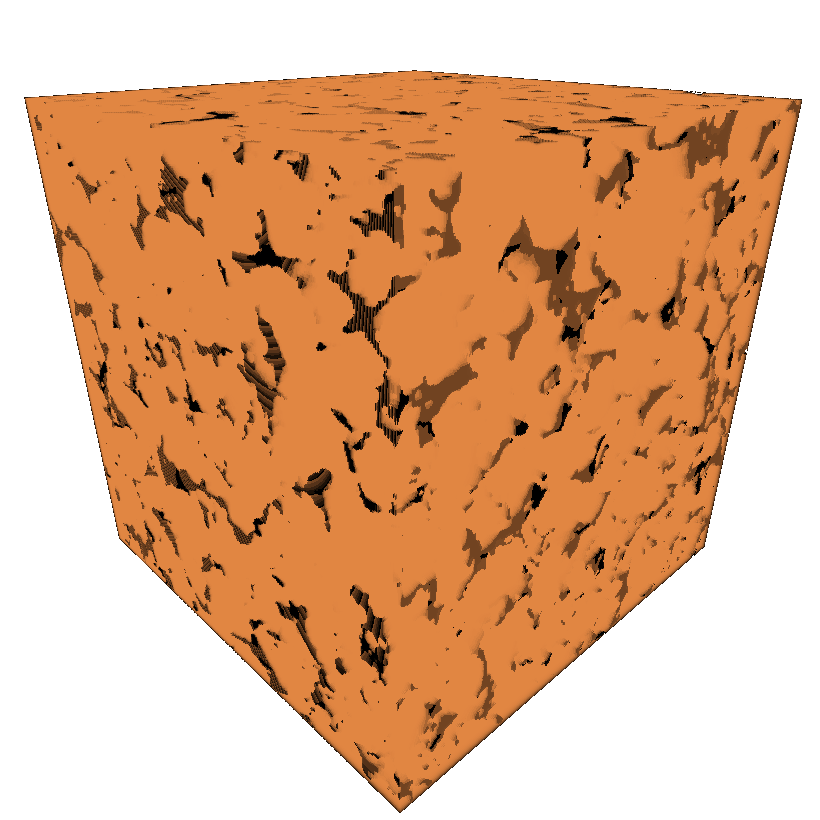
\includegraphics[width=0.3\linewidth]{images/sandstone3.png}
    \label{fig:sandstone3}}
  \vskip\baselineskip
  \subfigure[Carbonate 1, $C_{0.5} = 0.950$]{
    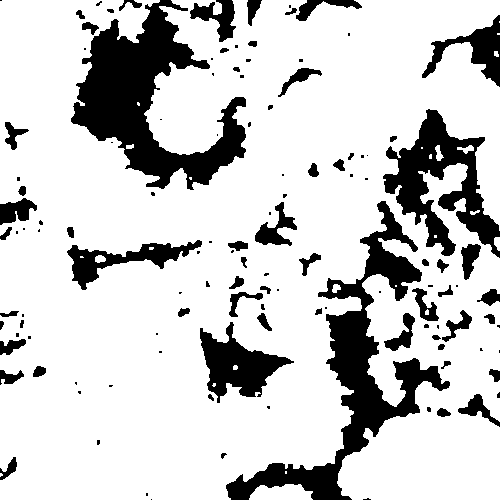
\includegraphics[width=0.3\linewidth]{images/carbonate1.png}
    \label{fig:carbonate1}}
  \hfill
  \subfigure[Carbonate 2, $C_{0.5} = 0.954$]{
    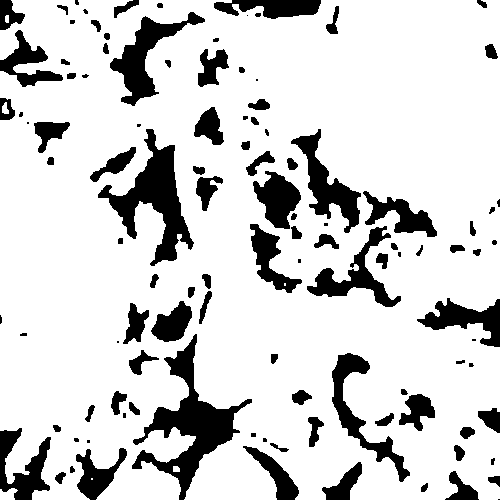
\includegraphics[width=0.3\linewidth]{images/carbonate2.png}
    \label{fig:carbonate2}}
  \hfill
  \subfigure[Carbonate 3, $C_{0.5} = 0.946$]{
    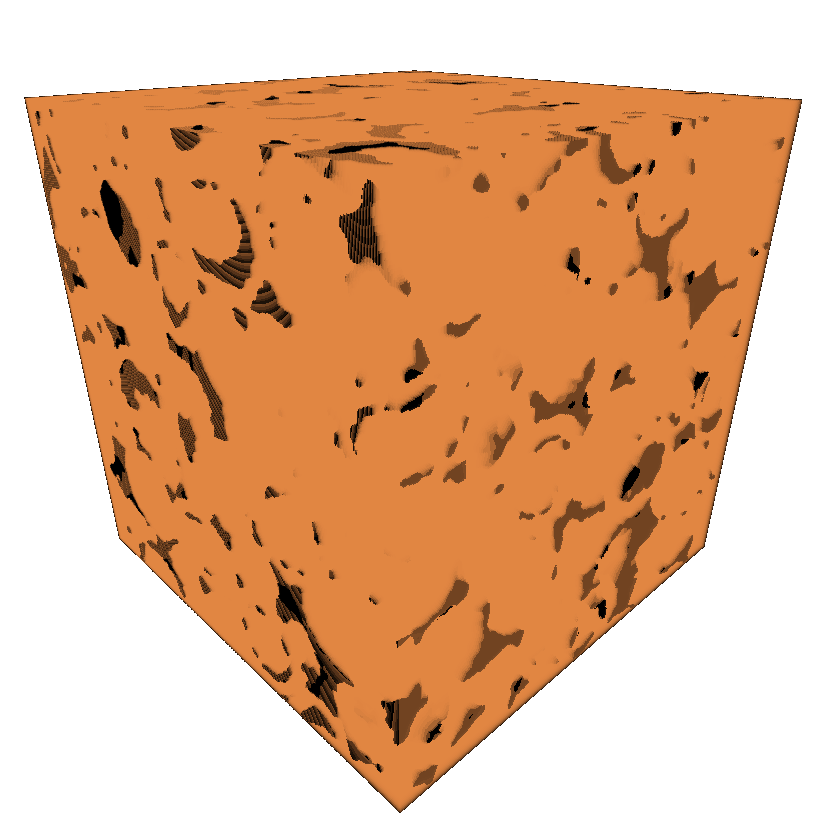
\includegraphics[width=0.3\linewidth]{images/carbonate3.png}
    \label{fig:carbonate3}}
  \caption[]{Data used in \cref{sec:application} for calculation of correlation
    functions.}
  \label{fig:real-data}
\end{figure*}

\begin{figure*}[t]
  \centering
  \subfigure[Surface-surface function]{
    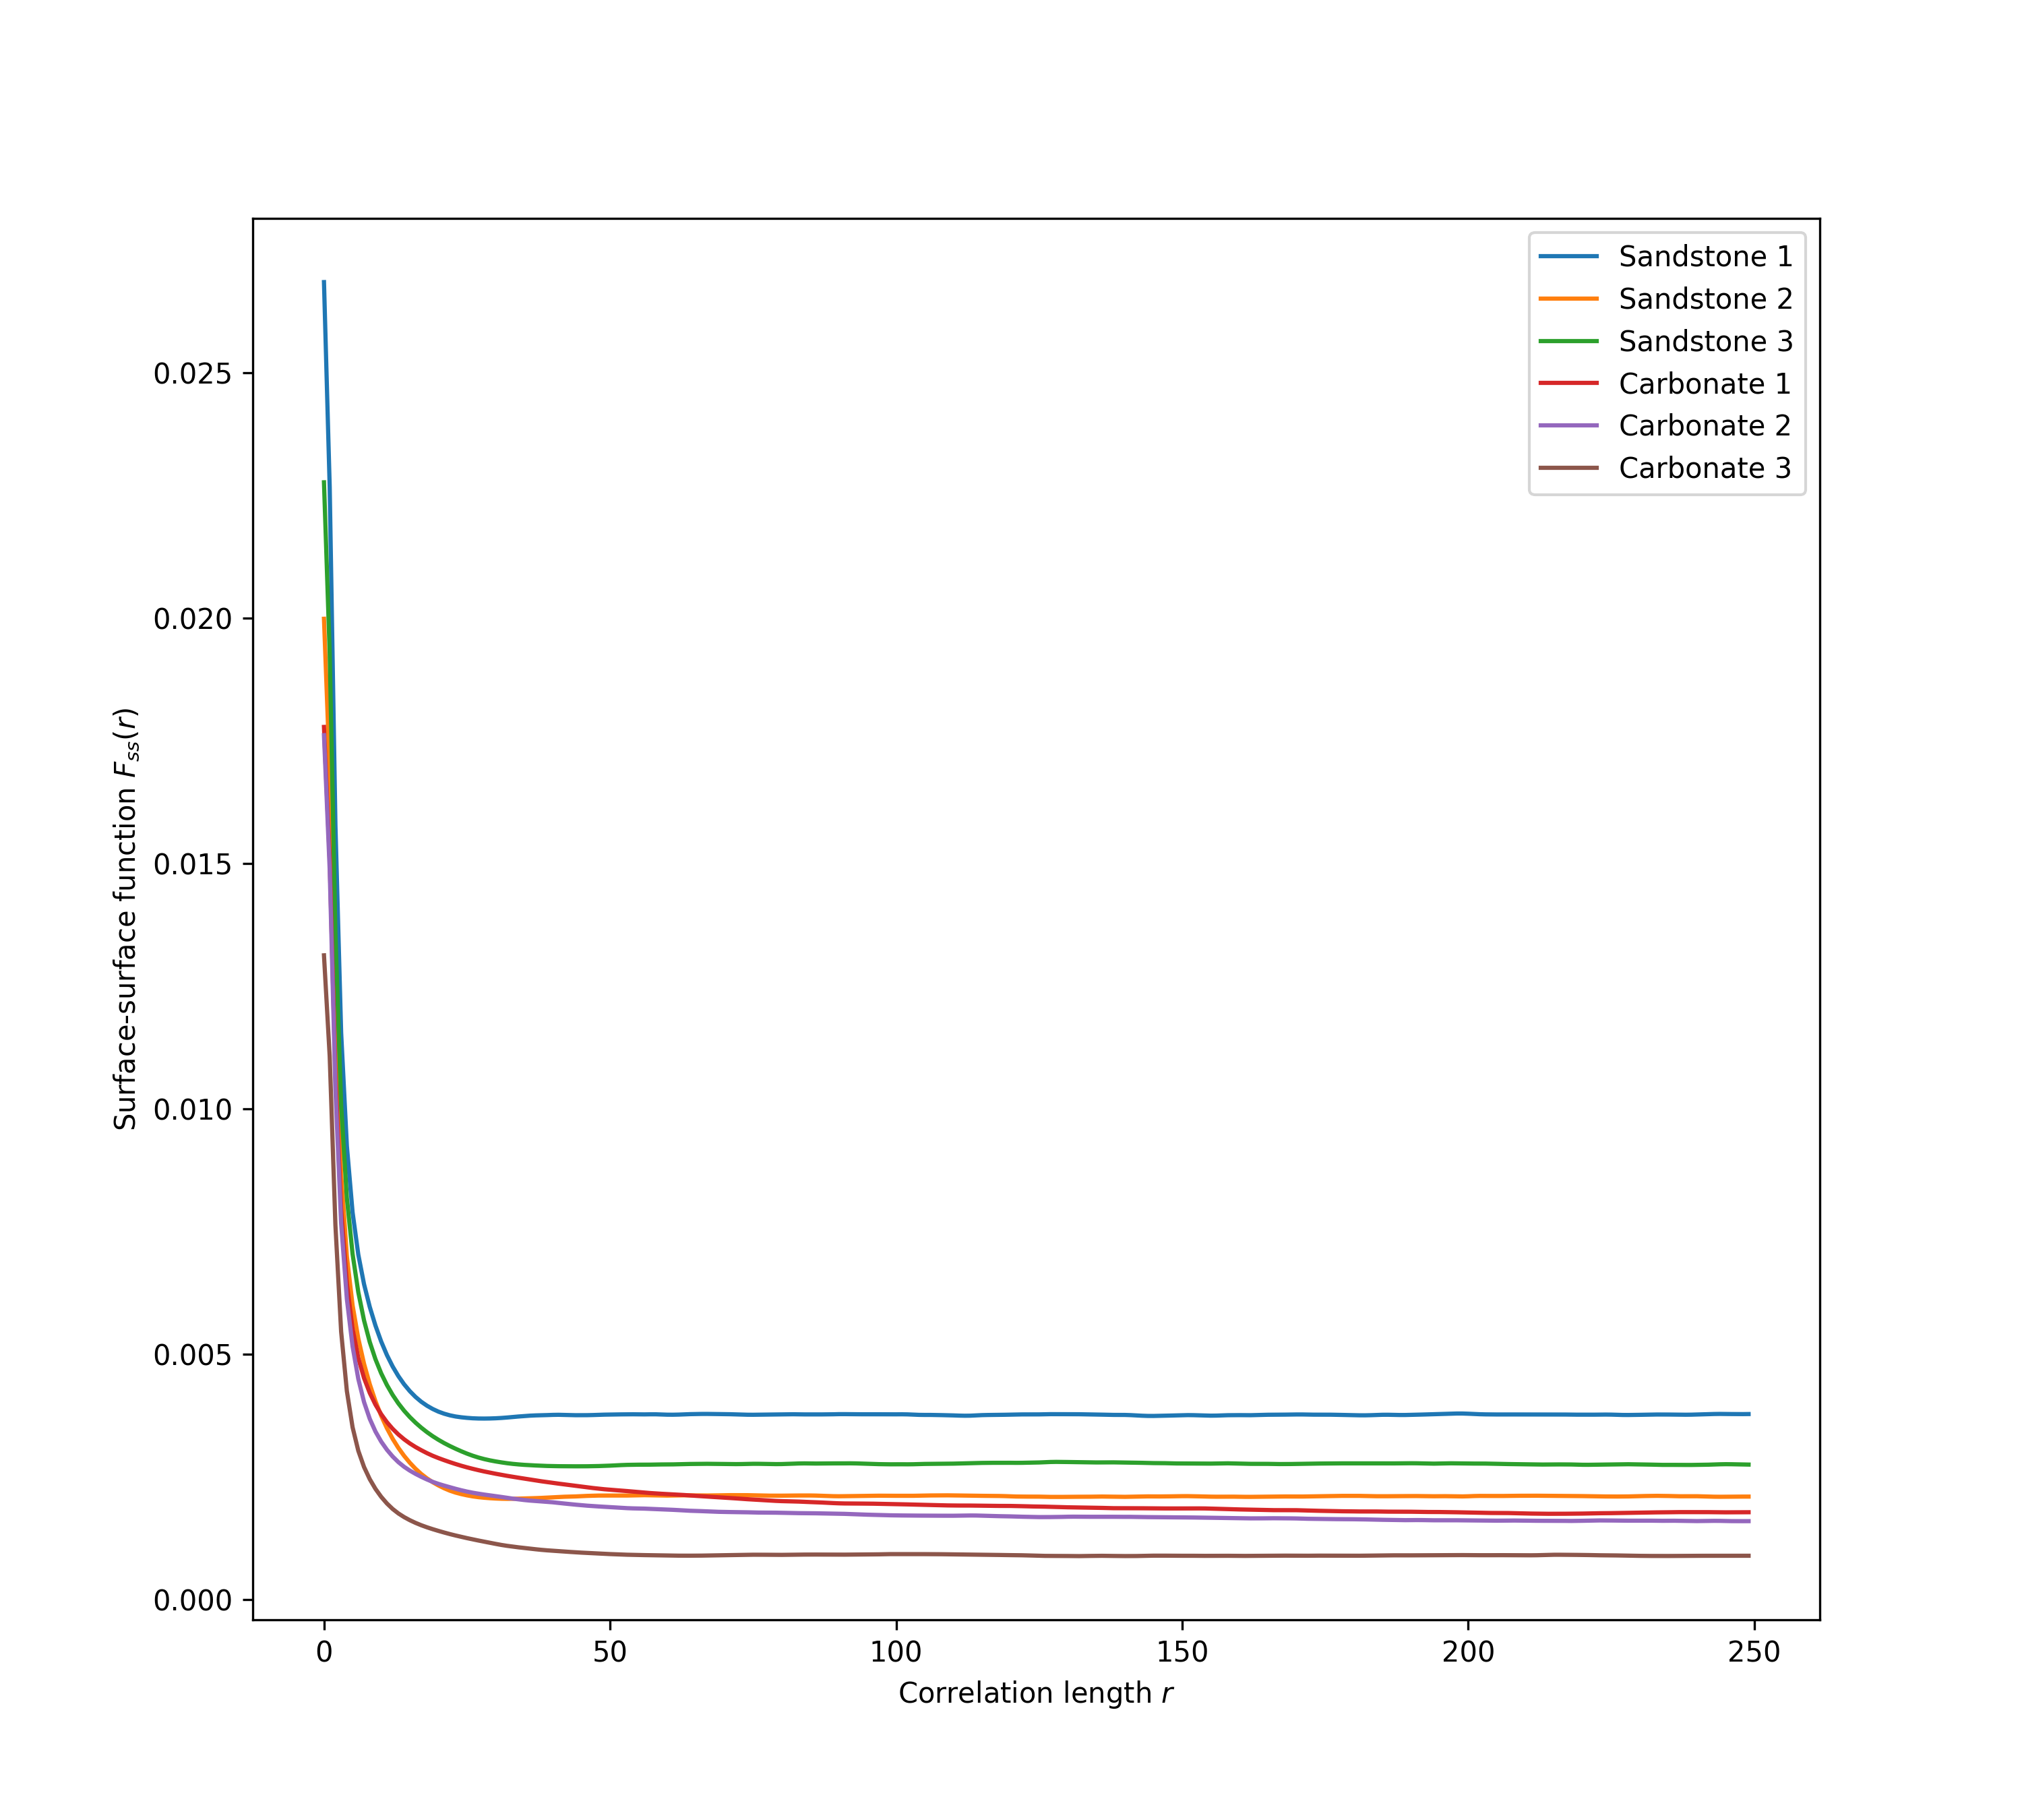
\includegraphics[width=0.475\linewidth]{images/KIK-ss.png}
    \label{fig:plot-ss-real}}
  \hfill
  \subfigure[Surface-void function]{
    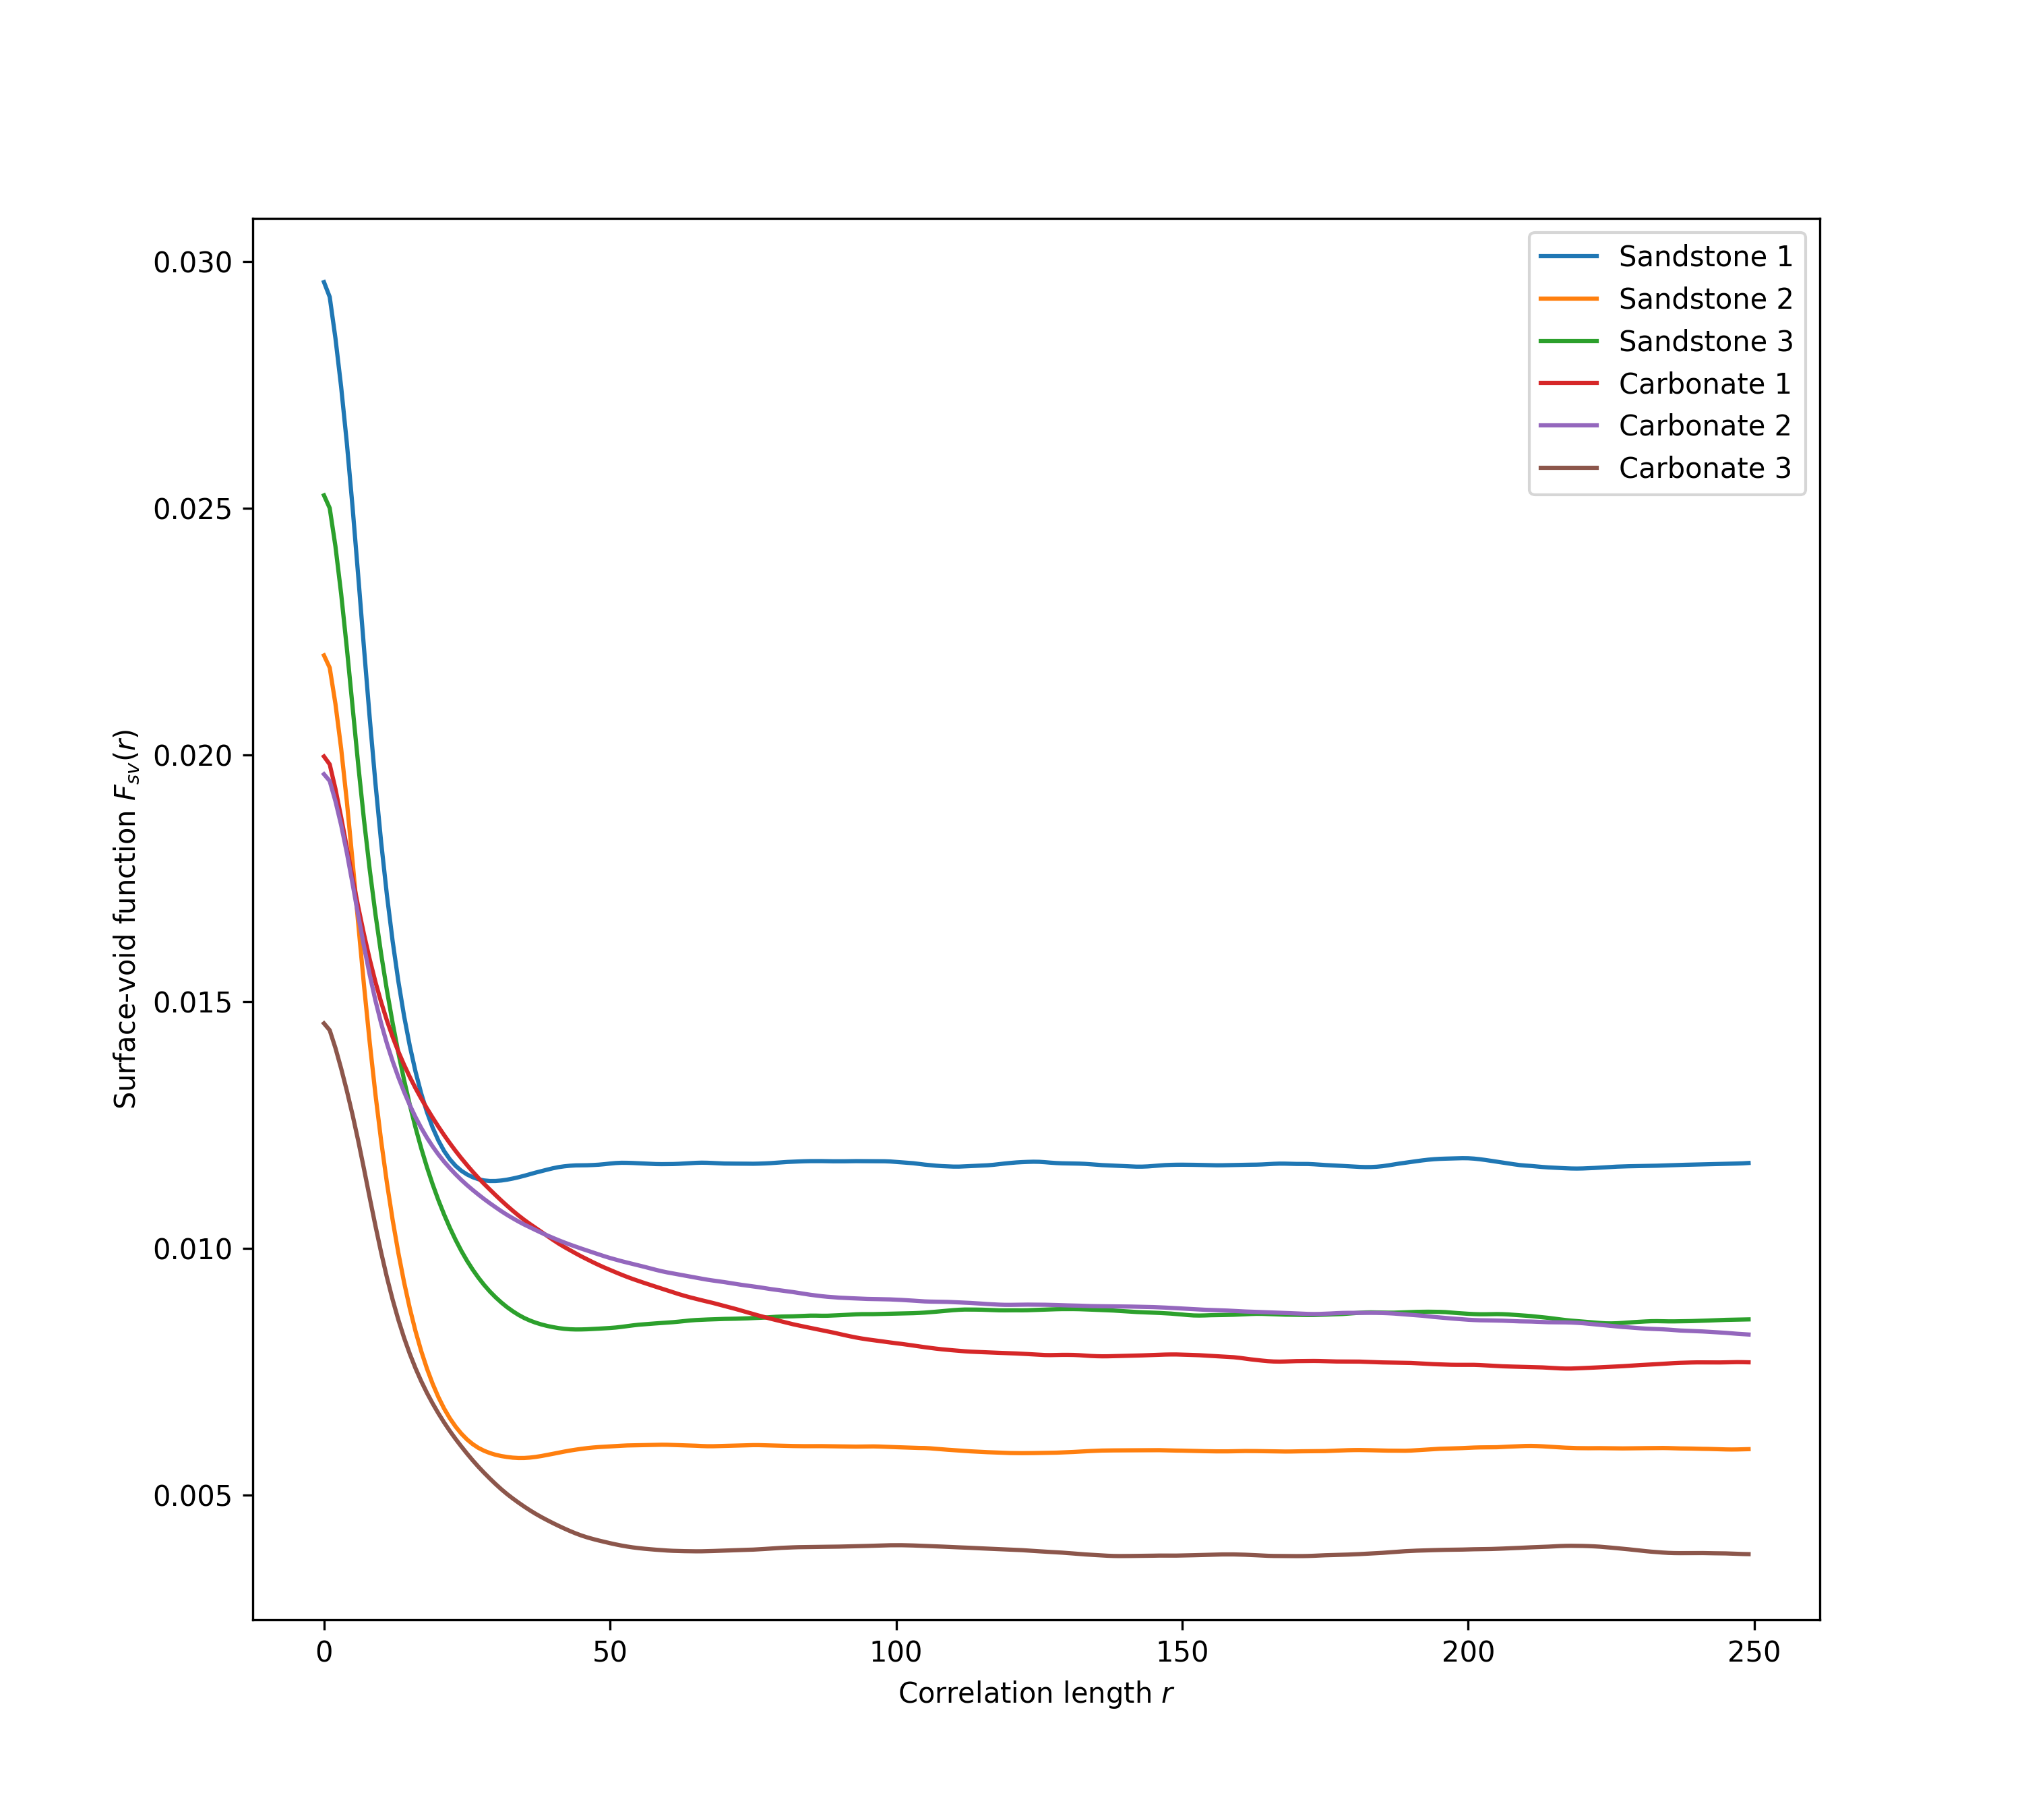
\includegraphics[width=0.475\linewidth]{images/KIK-sv.png}
    \label{fig:plot-sv-real}}
  \caption[]{Plots of $F_{ss}$ and $F_{sv}$ correlation functions computed for
    samples on \cref{fig:real-data}.}
  \label{fig:real-data-plots}
\end{figure*}

\begin{figure*}[t]
  \centering
  \subfigure[$C_{0.5} = 0.8397$]{
    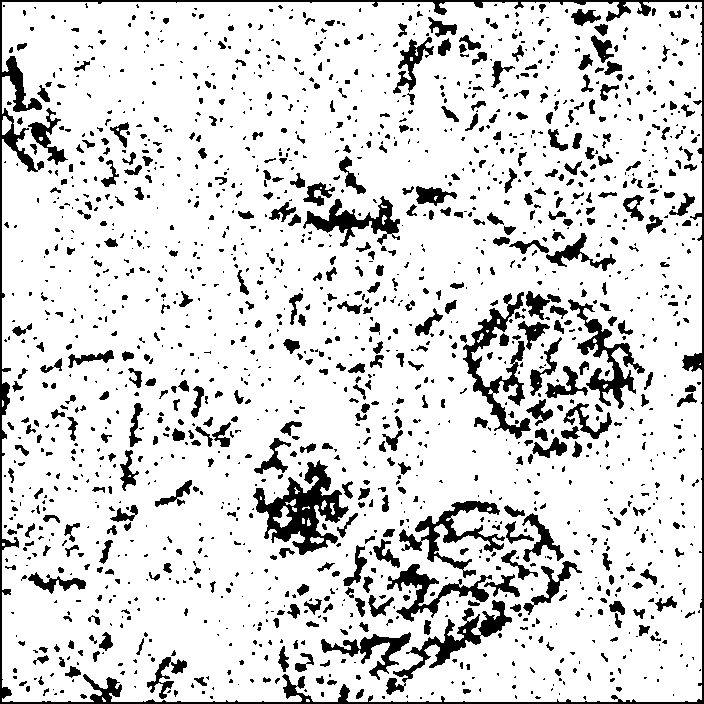
\includegraphics[width=0.475\linewidth]{images/sb-bad.png}
    \label{fig:bad1}}
  \hfill
  \subfigure[$C_{0.5} = 0.8517$]{
    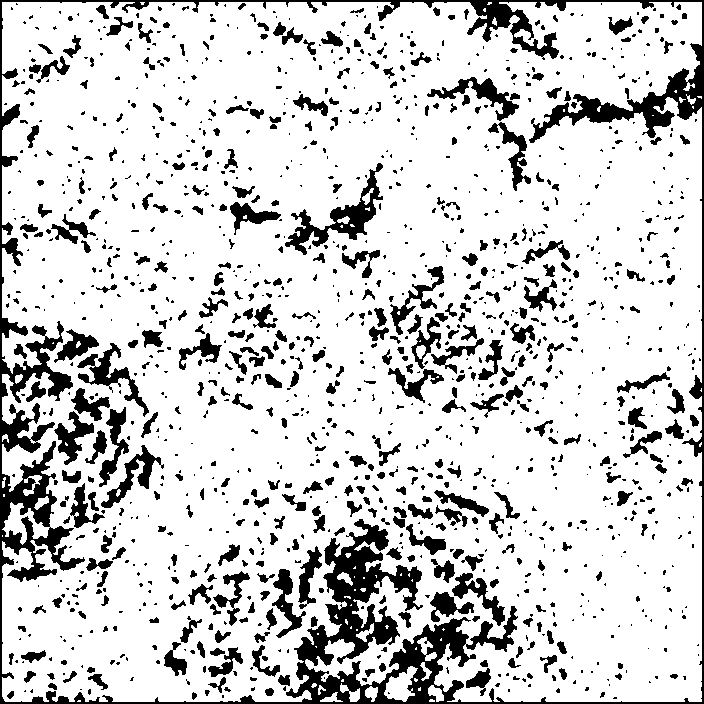
\includegraphics[width=0.475\linewidth]{images/sb-bad2.png}
    \label{fig:bad2}}
  \caption[]{Examples of images which do not pass $C_{0.5}$ criterion.}
  \label{fig:real-bad}
\end{figure*}

\section{Discussion and outline}
Exact vs. for-reconstruction computation of surface CFs

Our way it is easy to implement higher-order statistics computations, such as
multiple-point surface-surface correlation functions.

Discuss super-resolution to improve accuracy of surface functions computation
Explain that ``digital'' is better than ``continuous''.

\section{Conclusion}
Our summary says

\section{Acknowledgments}
This research was supported by the Russian Science Foundation grant
17-17-01310.

Collaborative effort of the authors within the FaT iMP (Flow and Transport in
Media with Pores) research group (www.porenetwork.com) and used some of its
software. We sincerely thank Prof. Salvatore Torquato for directing us to a
derivation of analytical formulas for 2D Poisson disks.

\appendix
\section{Derivation of analytical solutions for 2D Poisson disks}
\label{ap:overlapping-disks}
Analytic representation of surface-surface and surface-void correlation
functions for overlapping balls with centers generated by Poisson point process
is well known \cite{Torq_book}:
\begin{align}
  F_{sv}(r) &= -\lim_{a_1 \rightarrow R} \frac{\partial}{\partial a_1}
  e^{-\lambda S_{tot}(r, a_1, R)} \label{eq:fsv-disks} \\
  F_{ss}(r) &= -\lim_{a_1, a_2 \rightarrow R} \frac{\partial}{\partial a_1}
  \frac{\partial}{\partial a_2} e^{-\lambda S_{tot}(r, a_1,
    a_2)} \label{eq:fss-disks} \\
\end{align}
Here $S_{tot}(r, a_1, a_2)$ refers to a common volume of two n-dimensional balls
of radii $a_1$ and $a_2$ with a distance $r$ between their centers and $\lambda$
is a parameter of Poisson process. For two-dimensional disks we have the
following expression for $S_{tot}(r, a1, a2)$:
\begin{equation}
  S_{tot}(r, a_1, a_2) = \pi a_1^2 + \pi a_2^2 - S_{int}(r, a_1, a_2) \label{eq:total}
\end{equation}
where $S_{int}(r, a_1, a_2)$ is a common area of two disks, being equal to:
\cite{Math_stack_link}
\begin{align}
  S_{int}(r, a_1, a_2) =&  a_1^2 \arccos(\frac{r^2+a_1^2-a_2^2}{2a_1r}) + \\
  & a_2^2 \arccos(\frac{r^2+a_2^2-a_1^2}{2a_2r}) - \\
  & \frac{\sqrt{Y}}{2} \label{eq:intersection}
\end{align}
when $r<2R$ and zero otherwise. $Y$ in \cref{eq:intersection} is
\begin{equation*}
  Y = (-r+a_1+a_2)(r+a_2-a_1)(r+a_1-a_2)(r+a_1+a_2)
\end{equation*}
Substituting \cref{eq:intersection} into \cref{eq:total} and then
\cref{eq:total} into \cref{eq:fss-disks} we obtain \cref{eq:fss_final} for
$F_{ss}(r)$.

Similarly substituting \cref{eq:intersection} into \cref{eq:total} and then
\cref{eq:total} into \cref{eq:fsv-disks} we obtain \cref{eq:fsv_final} for
$F_{sv}(r)$.

\section{Implementation of surface function computations}
The code used to compute surface correlation functions in this manuscript was
written in Julia language and available as a Jupyter notebook in Supplementary
Materials. It uses \code{CorrelationFunctions.jl} package developed by our group
\cite{CorrFunc.jl_paper} that allows efficient computation of surface and other
correlation functions using both CPU and GPU architectures.

\section{Surface-surface correlation function for one disk}
The analytical representation of the surface-surface correlation function for
one disk is as follows:
\begin{equation*}
  F_{ss}(r) = \lim_{a_1, a_2 \rightarrow R} \frac{\partial}{\partial a_1}
  \frac{\partial}{\partial a_2} S_{tot}(r, a_1, a_2)
\end{equation*}
Following the same steps as in \cref{ap:overlapping-disks} we get a simple
formula:
\begin{equation*}
  F_{ss}(r,R) = \left\{
  \begin{array}{ll}
    \frac{4R^2}{r\sqrt{4R^2-r^2}} & \quad r < 2R \\
    0 & \quad \text{otherwise}
  \end{array} \right.
\end{equation*}
The resulting expression depends only on $t = r / 2R$:
\begin{equation*}
  F_{ss}(t) = \left\{
  \begin{array}{ll}
    \frac{1}{t\sqrt{1-t^2}} & \quad t < 1 \\
    0 & \quad \text{otherwise}
  \end{array} \right.
\end{equation*}
You can see that as $t$ tends to $0$ on the right or $1$ on the left,
$F_{ss}(t)$ tends to infinity.

\onecolumngrid
\bibliography{habib}
\bibliographystyle{plain}
\twocolumngrid

\end{document}
